\documentclass[12pt,a4paper,oneside]{report}

\usepackage[utf8]{inputenc}
\usepackage[vietnamese]{babel}
\usepackage[a4paper,left=3cm,right=2cm,top=2cm,bottom=2cm]{geometry}
\usepackage{graphicx}
\usepackage{amsmath,amssymb}
\usepackage{booktabs}
\usepackage{tabularx}
\usepackage{fancyhdr}
\usepackage{setspace}
\usepackage{listings}
\usepackage{xcolor}
\usepackage[colorlinks=true,linkcolor=blue!80!black,citecolor=green!60!black,urlcolor=blue]{hyperref}

% Header & Footer
\pagestyle{fancy}
\fancyhf{}
\fancyhead[R]{\small\textit{AIA331: Hệ thống Quản lý Kho có Tích hợp AI - Nhóm 11}}
\fancyfoot[C]{\thepage}
\fancyfoot[L]{\footnotesize\textit{Trường ĐH Công nghệ Thông tin \& Truyền thông - ĐHTN}}
\renewcommand{\headrulewidth}{0.5pt}
\renewcommand{\footrulewidth}{0.3pt}

\onehalfspacing
\graphicspath{{images/}}

\definecolor{codegray}{rgb}{0.5,0.5,0.5}
\definecolor{codepurple}{rgb}{0.58,0,0.82}
\definecolor{backcolour}{rgb}{0.96,0.97,0.98}

\lstdefinestyle{mystyle}{
    backgroundcolor=\color{backcolour},   
    commentstyle=\color{codegray},
    keywordstyle=\color{magenta},
    numberstyle=\tiny\color{codegray},
    stringstyle=\color{codepurple},
    basicstyle=\ttfamily\footnotesize,
    breakatwhitespace=false,         
    breaklines=true,                 
    captionpos=b,                    
    keepspaces=true,                 
    numbers=left,                    
    numbersep=5pt,                  
    showspaces=false,                
    showstringspaces=false,
    showtabs=false,                  
    tabsize=2
}
\lstset{style=mystyle}

\begin{document}

% ==================== 1. TRANG BÌA ====================
\begin{titlepage}
\begin{center}
    \textbf{\large ĐẠI HỌC THÁI NGUYÊN}\\[0.2cm]
    \textbf{\large TRƯỜNG ĐẠI HỌC CÔNG NGHỆ THÔNG TIN VÀ TRUYỀN THÔNG}\\[0.2cm]
    \textbf{------------------- o0o -------------------}\\[0.8cm]
    
    
\includegraphics[width=4.0cm]{logo_ictu.png}\\[0.8cm]
    
    \textbf{\Large BÁO CÁO DỰ ÁN HỌC PHẦN}\\[0.3cm]
    \textbf{\large HỌC PHẦN: ỨNG DỤNG TRÍ TUỆ NHÂN TẠO – AIA331}\\[0.2cm]
    \textbf{\small (MÃ HỌC PHẦN: 80273)}\\[1.0cm]
    
    \textbf{\LARGE HỆ THỐNG QUẢN LÝ KHO}\\[0.3cm]
    \textbf{\LARGE CÓ TÍCH HỢP TRÍ TUỆ NHÂN TẠO (AI)}\\[0.2cm]
    \textbf{\large (AI-POWERED SAAS INVENTORY MANAGEMENT SYSTEM)}\\[1.2cm]
\end{center}

\begin{flushleft}
\hspace{1.5cm}\begin{tabular}{ll}
    \textbf{Giảng viên hướng dẫn:} & \textbf{ThS. Nguyễn Tuấn Anh} \\[0.3cm]
    \textbf{Nhóm sinh viên thực hiện:} & \textbf{Nhóm 11} \\[0.2cm]
    \textbf{Sinh viên 1:} & Dương Minh Quang \hspace{0.5cm} MSV: DTC245200225 \\[0.2cm]
    \textbf{Sinh viên 2:} & Vũ Ngọc Anh Thuyên \hspace{0.3cm} MSV: DTC245200428 \\[0.2cm]
    \textbf{Ngành đào tạo:} & Công nghệ Thông tin - K24 ICTU
\end{tabular}
\end{flushleft}

\vfill
\begin{center}
    \textbf{THÁI NGUYÊN, THÁNG 09/2026}
\end{center}
\end{titlepage}

\pagenumbering{roman}

% ==================== 2. LỜI CẢM ƠN ====================
\chapter*{LỜI CẢM ƠN}
\addcontentsline{toc}{chapter}{LỜI CẢM ƠN}
Trong quá trình học tập, nghiên cứu và hoàn thành đồ án môn học ``Ứng dụng Trí tuệ Nhân tạo – AIA331'', nhóm 11 đã nhận được sự quan tâm, giảng dạy tận tình và hướng dẫn chi tiết từ Thầy ThS. Nguyễn Tuấn Anh – Giảng viên trực tiếp giảng dạy học phần. Thầy đã định hướng tư duy phân tích nghiệp vụ thực tế, kỹ nghệ thiết kế Prompt kiểm soát dữ liệu nền tảng và phương pháp xây dựng hệ thống phần mềm có độ tin cậy cao.

Nhóm cũng xin trân trọng cảm ơn Ban Giám hiệu, Khoa Công nghệ Thông tin – Trường Đại học Công nghệ Thông tin và Truyền thông, Đại học Thái Nguyên đã luôn tạo điều kiện thuận lợi về môi trường học tập và nghiên cứu.

\section*{Bảng phân công nhiệm vụ thành viên Nhóm 11}
\begin{table}[htbp]
\centering
\begin{tabularx}{\textwidth}{|c|X|c|X|c|}
\hline
\textbf{STT} & \textbf{Họ và Tên} & \textbf{Mã SV} & \textbf{Phần việc đảm nhiệm} & \textbf{Đóng góp} \\
\hline
1 & Dương Minh Quang & DTC245200225 & Trưởng nhóm: Kiến trúc 3 tầng, Backend FastAPI, ORM 11 bảng, Pipeline AI 2 lớp, Bộ test Pytest tự động. & 50\% \\
\hline
2 & Vũ Ngọc Anh Thuyên & DTC245200428 & Thành viên: Phân tích nghiệp vụ, Sơ đồ kỹ thuật (ERD, Use Case, Activity), Frontend React Vite SPA, Báo cáo kỹ thuật. & 50\% \\
\hline
\end{tabularx}
\caption{Bảng phân công nhiệm vụ và tỷ lệ đóng góp thành viên Nhóm 11}
\label{tab:mem}
\end{table}

\newpage

% ==================== 3. TÓM TẮT & TỪ KHÓA ====================
\chapter*{TÓM TẮT BÁO CÁO (ABSTRACT)}
\addcontentsline{toc}{chapter}{TÓM TẮT BÁO CÁO (ABSTRACT)}
Báo cáo trình bày kết quả nghiên cứu và xây dựng ``Hệ thống Quản lý Kho có Tích hợp Trí tuệ Nhân tạo (AI-Powered Inventory Management System)'' theo chuẩn kiến trúc 3 tầng phân tách: Presentation Tier (React 18 SPA, SaaS Dark Mode), Application Tier (FastAPI Async, Python 3.14), Data Tier (SQLAlchemy ORM 11 bảng CSDL chuẩn 3NF và dịch vụ đám mây Google Gemini 1.5 Flash).

Điểm nổi bật của đề tài là Pipeline AI 2 lớp (Dual-layer Resilience) kết hợp giữa Cloud LLM và Local Deterministic Rule Engine, giải quyết triệt để lỗi ZeroDivisionError và nguy cơ ảo giác số liệu (Anti-Hallucination) bằng kỹ thuật Ground-Truth Context Injection. Toàn bộ 12/12 ca kiểm thử tự động Backend (Pytest Suite) đạt tỷ lệ vượt qua 100\%, tích hợp phân quyền RBAC 3 vai trò và nhật ký kiểm toán Audit Logs bất biến.

\section*{TỪ KHÓA (KEYWORDS)}
\textit{Quản lý kho thông minh, Dual-layer AI Pipeline, Anti-Hallucination, Ground-Truth Context Injection, FastAPI, React Vite, SQLAlchemy ORM, RBAC, Pytest Automation, Audit Logs.}

\newpage

% ==================== 4. DANH MỤC TỪ VIẾT TẮT ====================
\chapter*{DANH MỤC CÁC TỪ VIẾT TẮT}
\addcontentsline{toc}{chapter}{DANH MỤC CÁC TỪ VIẾT TẮT}
\begin{table}[htbp]
\centering
\begin{tabularx}{\textwidth}{|l|X|X|}
\hline
\textbf{Từ viết tắt} & \textbf{Tên đầy đủ tiếng Anh} & \textbf{Diễn giải tiếng Việt} \\
\hline
AI & Artificial Intelligence & Trí tuệ Nhân tạo \\
API & Application Programming Interface & Giao diện lập trình ứng dụng \\
JWT & JSON Web Token & Chuỗi mã hóa xác thực người dùng không trạng thái \\
RBAC & Role-Based Access Control & Mô hình kiểm soát truy cập dựa trên vai trò \\
ORM & Object-Relational Mapping & Ánh xạ cơ sở dữ liệu quan hệ sang đối tượng \\
LLM & Large Language Model & Mô hình ngôn ngữ lớn (Google Gemini) \\
NLP & Natural Language Processing & Xử lý ngôn ngữ tự nhiên \\
SPA & Single Page Application & Ứng dụng web hiển thị động trên một trang \\
SKU & Stock Keeping Unit & Mã định danh đơn vị hàng hóa lưu kho \\
ERD & Entity Relationship Diagram & Sơ đồ thực thể liên kết cơ sở dữ liệu \\
\hline
\end{tabularx}
\caption{Danh mục các từ viết tắt chuyên ngành}
\label{tab:abbr}
\end{table}

\newpage

% ==================== 5. MỤC LỤC CHÍNH ====================
\tableofcontents
\newpage

% ==================== 6. MỤC LỤC CÁC BÀI KIỂM TRA KỸ NĂNG ====================
\chapter*{MỤC LỤC CÁC BÀI KIỂM TRA KỸ NĂNG}
\addcontentsline{toc}{chapter}{MỤC LỤC CÁC BÀI KIỂM TRA KỸ NĂNG}

Mục lục này giúp Giảng viên tra cứu trực tiếp các nội dung minh chứng cho từng bài kiểm tra kỹ năng của học phần AIA331 (Click vào từng mục để chuyển đến nội dung chi tiết):

\section*{\hypertarget{sec:kt1_toc}{BÀI KIỂM TRA THƯỜNG XUYÊN 1 – KT1 (PHÂN TÍCH \& THIẾT KẾ)}}
\begin{enumerate}
    \item \hyperlink{ch:01}{Phân tích đúng bài toán quản lý kho hàng} (Xem Chương~\ref{ch:01})
    \item \hyperlink{ch:02}{Xác định đầy đủ yêu cầu chức năng (FR01 - FR09)} (Xem Chương~\ref{ch:02})
    \item \hyperlink{ch:02}{Xác định yêu cầu phi chức năng (Bảo mật, Hiệu năng, ACID)} (Xem Chương~\ref{ch:02})
    \item \hyperlink{ch:03}{Thiết kế actor và sơ đồ Use Case tổng thể} (Xem Chương~\ref{ch:03})
    \item \hyperlink{ch:05}{Thiết kế cơ sở dữ liệu quan hệ chuẩn hóa 3NF (11 Bảng)} (Xem Chương~\ref{ch:05})
    \item \hyperlink{ch:06}{Thiết kế kiến trúc hệ thống 3 tầng phân tách độc lập} (Xem Chương~\ref{ch:06})
    \item \hyperlink{ch:08}{Xác định vị trí ứng dụng AI giải quyết bài toán cạn tồn} (Xem Chương~\ref{ch:08})
    \item \hyperlink{ch:09}{Thiết kế prompt và luồng gọi AI có kiểm soát dữ liệu} (Xem Chương~\ref{ch:09})
    \item \hyperlink{ch:13}{Minh chứng sử dụng AI hỗ trợ phân tích thiết kế} (Xem Chương~\ref{ch:13})
    \item \hyperlink{ch:14}{Hồ sơ tài liệu phân tích thiết kế kỹ thuật hoàn chỉnh} (Xem Chương~\ref{ch:14})
\end{enumerate}

\section*{\hypertarget{sec:kt2_toc}{BÀI KIỂM TRA THƯỜNG XUYÊN 2 – KT2 (BACKEND, CSDL \& BẢO MẬT)}}
\begin{enumerate}
    \item \hyperlink{ch:06}{Cấu trúc dự án mã nguồn theo nguyên lý Clean Architecture} (Xem Chương~\ref{ch:06})
    \item \hyperlink{ch:11}{Đăng nhập an toàn và phân quyền RBAC 3 vai trò} (Xem Chương~\ref{ch:11})
    \item \hyperlink{ch:07}{CRUD nghiệp vụ quản lý sản phẩm, vị trí kệ và giao dịch} (Xem Chương~\ref{ch:07})
    \item \hyperlink{ch:07}{Tìm kiếm và lọc hàng hóa thông minh, hiển thị trạng thái tồn kho} (Xem Chương~\ref{ch:07})
    \item \hyperlink{ch:07}{Thống kê và báo cáo tài chính kho (KPIs, định giá kho)} (Xem Chương~\ref{ch:07})
    \item \hyperlink{ch:15}{Giao diện người dùng SaaS Dark Mode hiện đại trực quan} (Xem Chương~\ref{ch:15})
    \item \hyperlink{ch:05}{Kết nối CSDL quan hệ SQLAlchemy ORM 11 bảng} (Xem Chương~\ref{ch:05})
    \item \hyperlink{ch:10}{Xử lý lỗi toàn cục và bắt ngoại lệ HTTP an toàn} (Xem Chương~\ref{ch:10})
    \item \hyperlink{ch:13}{Minh chứng sử dụng AI hỗ trợ lập trình và tối ưu hóa} (Xem Chương~\ref{ch:13})
    \item \hyperlink{ch:12}{README và tài liệu hướng dẫn vận hành, chạy thử} (Xem Chương~\ref{ch:12})
\end{enumerate}

\section*{\hypertarget{sec:kt3_toc}{BÀI KIỂM TRA THƯỜNG XUYÊN 3 – KT3 (TÍCH HỢP TRÍ TUỆ NHÂN TẠO)}}
\begin{enumerate}
    \item \hyperlink{ch:08}{Tích hợp giải pháp AI giải quyết bài toán quản lý kho} (Xem Chương~\ref{ch:08})
    \item \hyperlink{ch:08}{Kết nối API Cloud LLM (Gemini) và Bộ máy Rule Engine cục bộ} (Xem Chương~\ref{ch:08})
    \item \hyperlink{ch:09}{Thiết kế Prompt có cấu trúc nghiêm ngặt định dạng Markdown} (Xem Chương~\ref{ch:09})
    \item \hyperlink{ch:09}{Tối ưu prompt và cơ chế chống ảo giác số liệu (Anti-Hallucination)} (Xem Chương~\ref{ch:09})
    \item \hyperlink{ch:09}{Sử dụng dữ liệu thực tế hệ thống (Ground-Truth Context Injection)} (Xem Chương~\ref{ch:09})
    \item \hyperlink{ch:08}{Hiển thị kết quả AI dạng Smart Component kèm bảng số liệu} (Xem Chương~\ref{ch:08})
    \item \hyperlink{ch:08}{Xử lý lỗi, ngắt kết nối mạng và chuyển vùng dự phòng cục bộ} (Xem Chương~\ref{ch:08})
    \item \hyperlink{ch:10}{Kiểm thử tự động các chức năng AI (Restock, Anomaly, NLP Chat)} (Xem Chương~\ref{ch:10})
    \item \hyperlink{ch:13}{Review mã nguồn tự động và giám sát chất lượng bằng AI} (Xem Chương~\ref{ch:13})
    \item \hyperlink{ch:15}{Tích hợp AI nâng cao trải nghiệm người vận hành kho} (Xem Chương~\ref{ch:15})
\end{enumerate}

\section*{\hypertarget{sec:ck_toc}{THI KẾT THÚC HỌC PHẦN (HOÀN THIỆN ĐỒ ÁN \& ĐÓNG GÓI)}}
\begin{enumerate}
    \item \hyperlink{ch:07}{Hoàn thiện toàn bộ chức năng nghiệp vụ hệ thống} (Xem Chương~\ref{ch:07})
    \item \hyperlink{ch:06}{Chất lượng kiến trúc hệ thống và tính module hóa mã nguồn} (Xem Chương~\ref{ch:06})
    \item \hyperlink{ch:05}{Chất lượng cơ sở dữ liệu chuẩn 3NF và tính toàn vẹn ACID} (Xem Chương~\ref{ch:05})
    \item \hyperlink{ch:15}{Giao diện và trải nghiệm người dùng chuyên nghiệp (SaaS UI)} (Xem Chương~\ref{ch:15})
    \item \hyperlink{ch:08}{Chất lượng bộ máy AI kép hoạt động ổn định và chính xác} (Xem Chương~\ref{ch:08})
    \item \hyperlink{ch:11}{Bảo mật OWASP, quyền riêng tư dữ liệu và đạo đức AI} (Xem Chương~\ref{ch:11})
    \item \hyperlink{ch:10}{Hiệu năng xử lý cao và bộ kiểm thử 100\% Passed} (Xem Chương~\ref{ch:10})
    \item \hyperlink{ch:12}{Triển khai, đóng gói và cung cấp sẵn Seed Data thử nghiệm} (Xem Chương~\ref{ch:12})
    \item \hyperlink{ch:14}{Hồ sơ báo cáo kỹ thuật hoàn chỉnh (Word chuẩn Bộ \& LaTeX)} (Xem Chương~\ref{ch:14})
    \item \hyperlink{ch:15}{Kịch bản thuyết trình và chạy thử nghiệm hệ thống (Demo)} (Xem Chương~\ref{ch:15})
\end{enumerate}

\newpage

% ==================== 7. DANH MỤC HÌNH & BẢNG ====================
\listoffigures
\newpage
\listoftables
\newpage

% ==================== 8. BẢNG TRA CỨU 40 TIÊU CHÍ ====================
\chapter*{BẢNG TRA CỨU NỘI DUNG THEO BÀI KIỂM TRA}
\addcontentsline{toc}{chapter}{BẢNG TRA CỨU NỘI DUNG THEO BÀI KIỂM TRA}

\begin{table}[htbp]
\centering
\small
\begin{tabularx}{\textwidth}{|c|X|c|X|X|}
\hline
\textbf{Bài KT} & \textbf{Tiêu chí kiểm tra} & \textbf{Chương/Mục} & \textbf{Minh chứng} & \textbf{File / Mã nguồn} \\
\hline
KT1 & 1. Phân tích bài toán quản lý & Ch.1 (1.1) & Ngữ cảnh kho SME & services/ (kho) \\
KT1 & 2. Yêu cầu chức năng FR01-09 & Ch.2 (2.1) & Bảng 2.1 FR01-09 & models/ (specs) \\
KT1 & 3. Yêu cầu phi chức năng & Ch.2 (2.2) & ACID, OWASP & core/security.py \\
KT1 & 4. Actor \& Use Case tổng thể & Ch.3 (3.1) & Hình 3.1 Use Case & routers/ \\
KT1 & 5. Thiết kế CSDL chuẩn 3NF & Ch.5 (5.1) & Hình 5.1 ERD 11 bảng & database.py \\
KT1 & 6. Kiến trúc hệ thống 3 tầng & Ch.6 (6.1) & Hình 6.1 Kiến trúc & app/ \& src/ \\
KT1 & 7. Vị trí ứng dụng AI & Ch.8 (8.1) & Hình 8.1 Pipeline AI & ai/gemini.py \\
KT1 & 8. Thiết kế prompt có cấu trúc & Ch.9 (9.1) & System Prompt & ai/prompts.py \\
KT1 & 9. Minh chứng dùng AI SDLC & Ch.13 (13.1)& AI Assistant Log & tests/ai\_logs/ \\
KT1 & 10. Tài liệu phân tích hoàn chỉnh & Ch.1-6 & 10 bản vẽ kỹ thuật & docs/ \\
\hline
KT2 & 1. Cấu trúc Clean Architecture & Ch.6 \& Ch.7 & backend/ \& frontend/ & routers/, services/ \\
KT2 & 2. Đăng nhập \& RBAC 3 vai trò & Ch.11 (11.2) & Bảng 11.1 Ma trận RBAC & middleware/auth.py \\
KT2 & 3. CRUD nghiệp vụ kho & Ch.7 (7.1-7.2)& API Products \& Trans & api/v1/endpoints/ \\
KT2 & 4. Tìm kiếm và lọc hàng hóa & Ch.7 (7.3) & Smart Table Search & InventoryTable.jsx \\
KT2 & 5. Thống kê báo cáo tài chính & Ch.7 (7.4) & Hình 15.1 Thẻ 6 KPI & AnalyticsView.jsx \\
KT2 & 6. Giao diện SaaS Dark Mode & Ch.15 & SaaS UI HorizonX & Tailwind CSS \\
KT2 & 7. CSDL SQLAlchemy ORM & Ch.5 (5.3) & Bảng 5.1 11 Model & models/entities.py \\
KT2 & 8. Xử lý ngoại lệ HTTP an toàn & Ch.10 (10.3) & Exception Handlers & main.py \\
KT2 & 9. Minh chứng AI lập trình & Ch.13 (13.2) & Sinh Test \& Query & tests/test\_api.py \\
KT2 & 10. README và hướng dẫn chạy & Ch.12 (12.2) & Hướng dẫn Uvicorn/npm & README.md \\
\hline
KT3 & 1. Tích hợp AI bài toán kho & Ch.8 (8.1) & Dự báo cạn tồn & ai/depletion.py \\
KT3 & 2. Kết nối Cloud \& Local AI & Ch.8 (8.2-8.3)& Dual-layer Pipeline & ai/pipeline.py \\
KT3 & 3. Thiết kế Prompt có cấu trúc & Ch.9 (9.1) & Markdown Prompt & ai/templates.py \\
KT3 & 4. Cơ chế chống ảo giác & Ch.9 (9.2) & Anti-Hallucination & services/guard.py \\
KT3 & 5. Dữ liệu thực tế hệ thống & Ch.9 (9.3) & Ground-Truth Context & ai/context.py \\
KT3 & 6. Hiển thị kết quả AI & Ch.8 \& Ch.15& Hình 15.3 AI Hub & AiInsights.jsx \\
KT3 & 7. Xử lý ngắt mạng dự phòng & Ch.8 (8.3) & Local Rule Engine & ai/rule\_engine.py \\
KT3 & 8. Kiểm thử chức năng AI & Ch.10 (10.2) & TC10, TC11, TC12 & tests/test\_ai.py \\
KT3 & 9. Review code bằng AI & Ch.13 (13.3) & Review Log tự động & .agent/review.log \\
KT3 & 10. Trải nghiệm người dùng AI & Ch.15 (15.2) & Hình 15.4 Chat Console & AiChatModal.jsx \\
\hline
CK & 1-10. Đồ án hoàn chỉnh & Ch.1 - Ch.16 & 16 Chương, 100\% Test & Full Codebase \\
\hline
\end{tabularx}
\caption{Bảng tra cứu nội dung minh chứng theo 40 tiêu chí kiểm tra môn học}
\label{tab:matrix}
\end{table}

\newpage
\pagenumbering{arabic}

% ==================== 16 CHƯƠNG KỸ THUẬT ====================
\chapter{TỔNG QUAN ĐỀ TÀI}
\label{ch:01}

\section{Bối cảnh bài toán quản lý kho tại các doanh nghiệp vừa và nhỏ}
Trong chuỗi cung ứng hiện đại, kho bãi giữ vai trò mạch máu lưu chuyển dòng vật chất và vốn của doanh nghiệp. Qua quá trình khảo sát thực tế tại các đơn vị phân phối linh kiện máy tính và thiết bị mạng, các doanh nghiệp vừa và nhỏ (SMEs) thường gặp phải các hạn chế nghiêm trọng do sử dụng sổ tay hoặc Excel phân tán: độ trễ thông tin từ 1 đến 3 ngày, nguy cơ sai sót cao và tình trạng chôn vốn lưu động.

\section{Mục tiêu, đối tượng và phạm vi nghiên cứu}
Đề tài hướng tới xây dựng hệ thống Quản lý Kho thông minh có tích hợp Trí tuệ Nhân tạo, tự động hóa xuất nhập tồn, phân tích vận tốc tiêu thụ và cung cấp trợ lý hỏi đáp tự nhiên. Đối tượng áp dụng là các nhà kho phân phối quy mô vừa với phân quyền 3 vai trò: Quản trị viên, Thủ kho và Kế toán.

\section{Phương pháp nghiên cứu và cách tiếp cận ứng dụng AI}
Ứng dụng nguyên tắc Chống ảo giác dữ liệu (Anti-Hallucination) với Ground-Truth Context Injection và xây dựng kiến trúc dự phòng kép (Dual-layer Resilience) đảm bảo hệ thống luôn hoạt động liên tục.

\chapter{PHÂN TÍCH YÊU CẦU}
\label{ch:02}

\section{Yêu cầu chức năng chi tiết (FR01 - FR09)}
Hệ thống đáp ứng đầy đủ 9 nhóm yêu cầu chức năng cốt lõi:
\begin{itemize}
    \item \textbf{FR01 - Xác thực \& RBAC:} Đăng nhập JWT Bearer, phân quyền 3 vai trò.
    \item \textbf{FR02 - Dữ liệu nền tảng:} Quản lý danh mục, nhà cung cấp, sơ đồ kệ kho.
    \item \textbf{FR03 - Quản lý Sản phẩm:} Quản lý SKU, giá vốn, giá bán, định mức an toàn.
    \item \textbf{FR04 - Giao dịch Nhập kho:} Lập phiếu nhập, kiểm đếm thực tế, gán vị trí ô kệ.
    \item \textbf{FR05 - Giao dịch Xuất kho:} Lập phiếu xuất, kiểm tra tồn khả dụng, khóa an toàn.
    \item \textbf{FR06 - Dự báo Tồn kho AI:} Tính Burn-rate, Depletion Days và gợi ý tái nhập.
    \item \textbf{FR07 - Phát hiện Bất thường AI:} Kiểm định thống kê Z-score phát hiện giao dịch lạ.
    \item \textbf{FR08 - Trợ lý Hỏi Đáp Kho AI:} Hộp thoại NLP hỏi đáp tồn kho bằng tiếng Việt.
    \item \textbf{FR09 - Nhật ký Kiểm toán:} Ghi vết bất biến mọi thao tác C/U/D trong hệ thống.
\end{itemize}

\section{Yêu cầu phi chức năng}
Bảo mật OWASP Top 10, thời gian đáp ứng API $<100$ms, thực thi giao dịch nguyên tử ACID và giao diện SaaS Dark Mode trực quan.

\chapter{PHÂN TÍCH ACTOR VÀ USE CASE}
\label{ch:03}

\section{Xác định và phân quyền 3 tác nhân Actor}
Hệ thống phân định 3 tác nhân: Quản trị viên (Admin), Thủ kho (Warehouse Staff) và Kế toán kho (Accountant).

\section{Sơ đồ Use Case tổng thể hệ thống}
Sơ đồ Use Case tổng thể được trình bày tại Hình~\ref{fig:usecase}.

\begin{figure}[htbp]
    \centering
    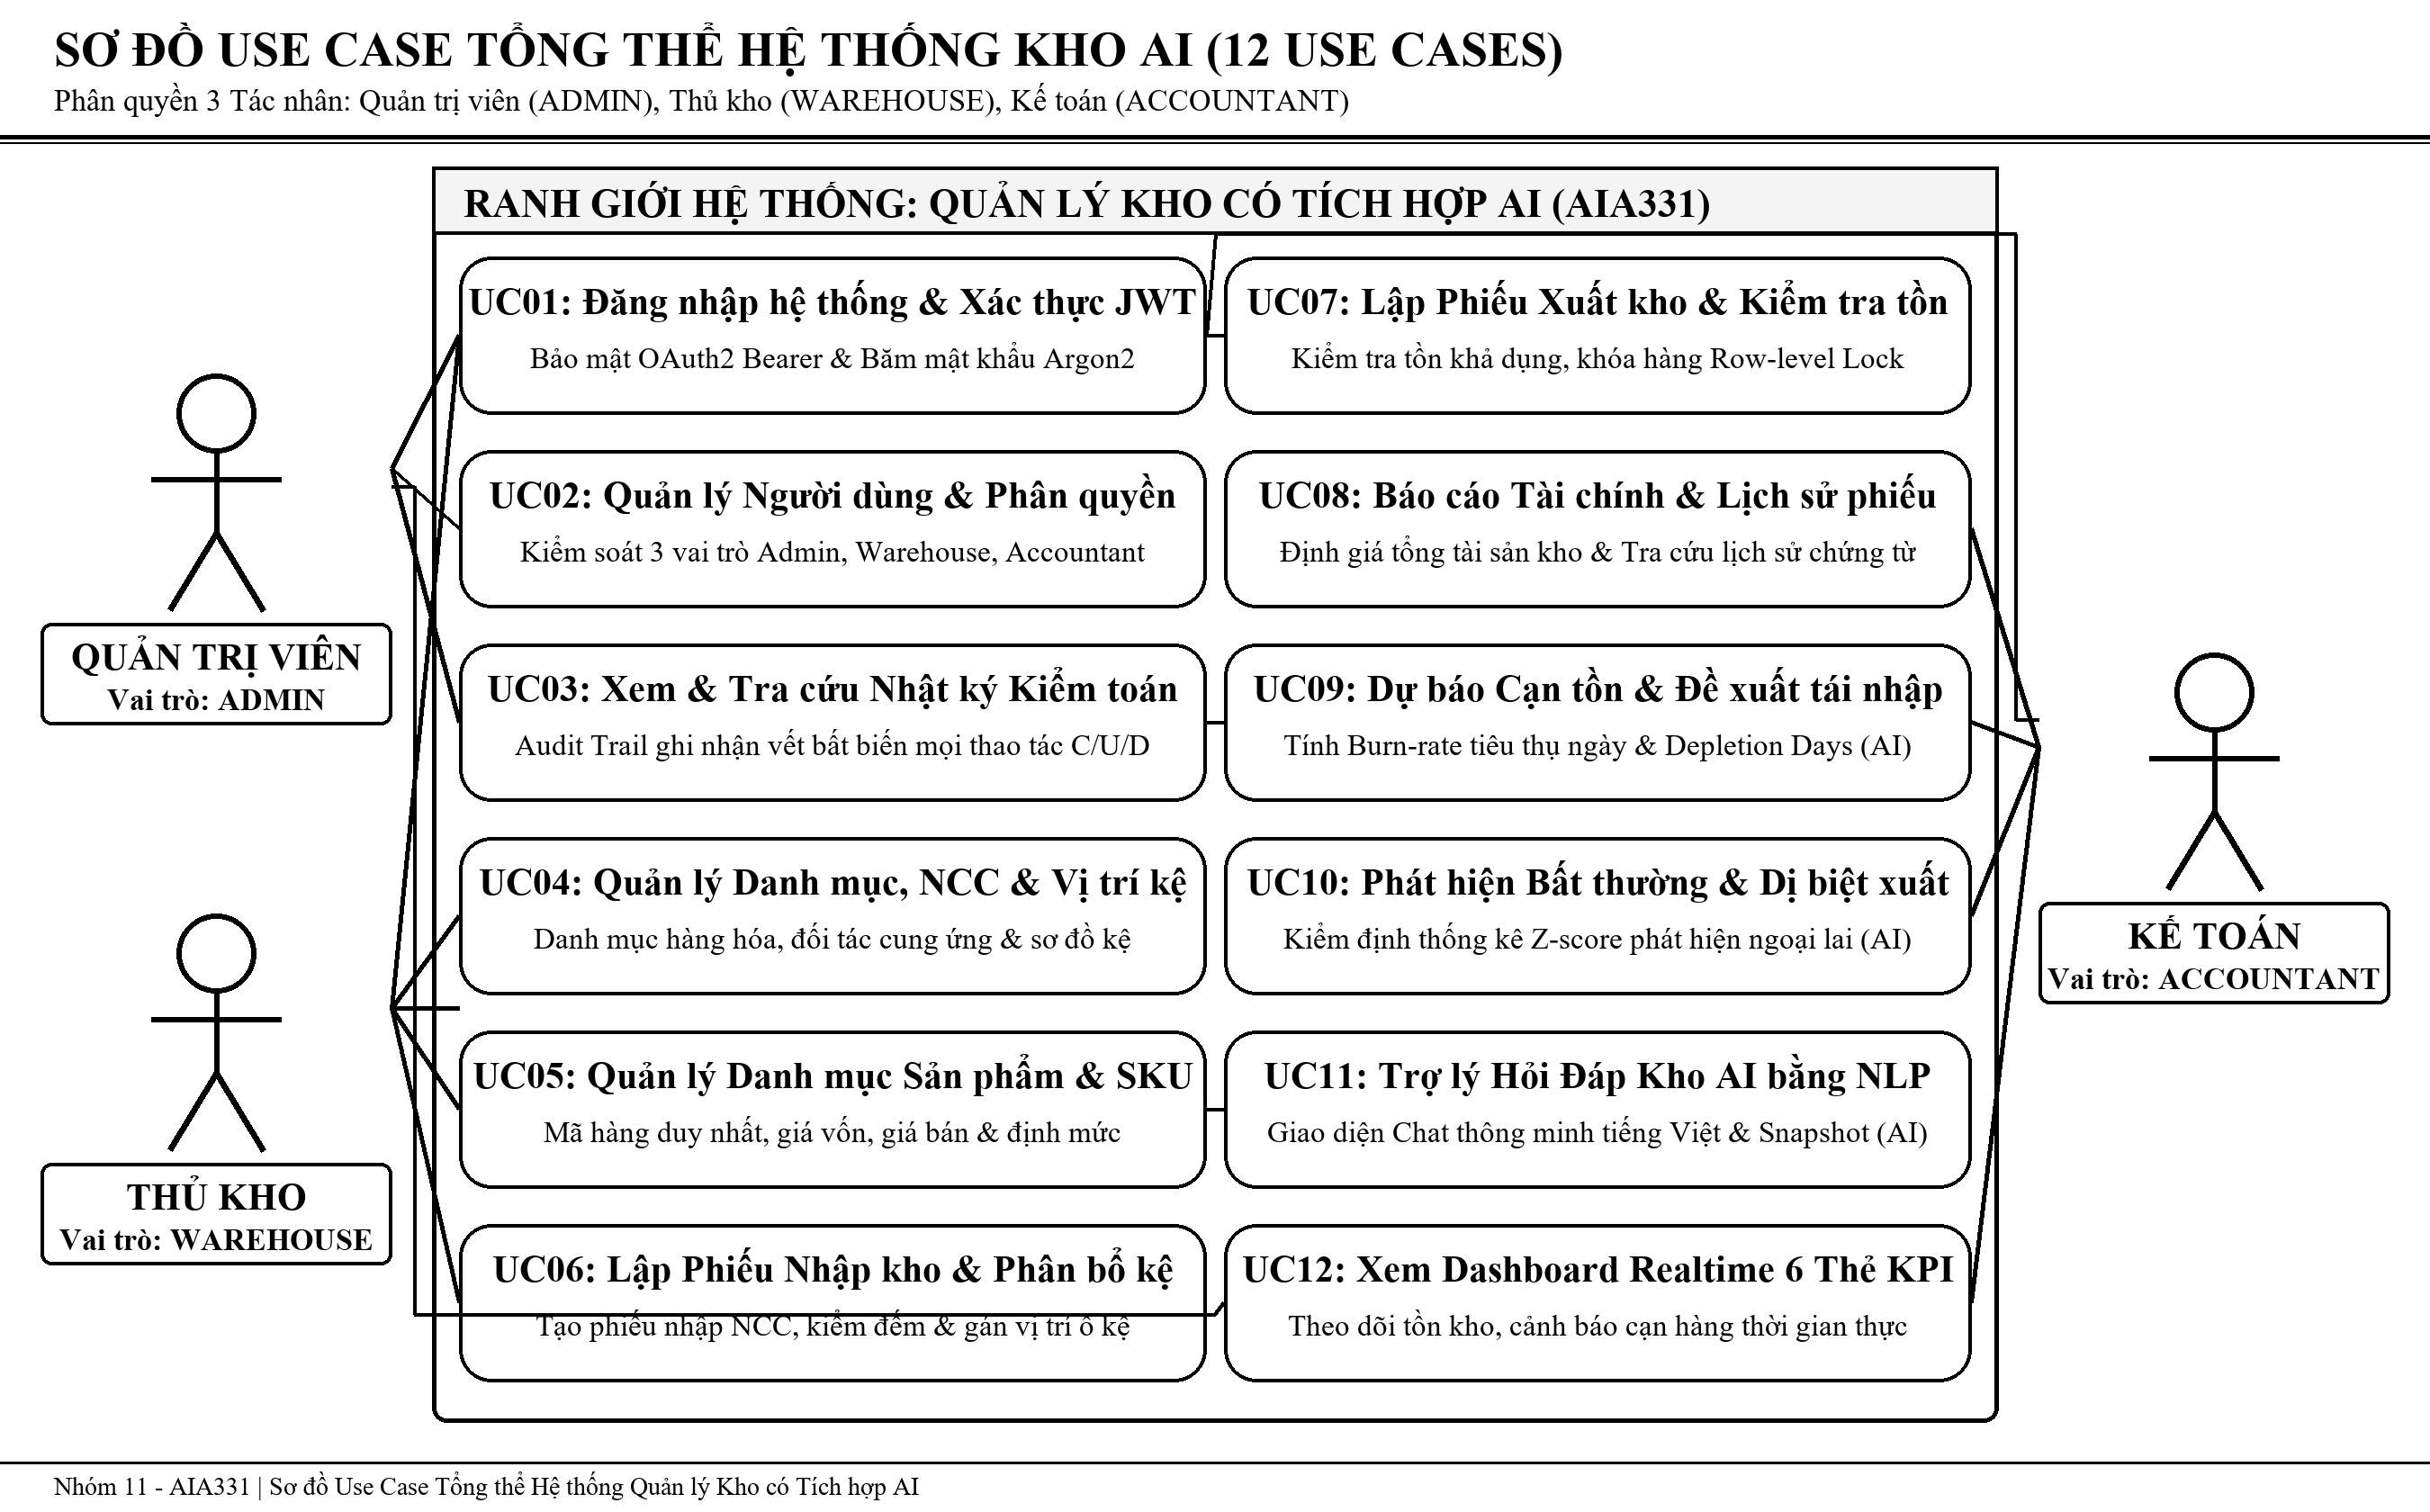
\includegraphics[width=0.92\textwidth]{02_so_do_usecase_tong_the.png}
    \caption{Sơ đồ Use Case tổng thể hệ thống phân quyền 3 tác nhân (Nhóm 11)}
    \label{fig:usecase}
\end{figure}

\chapter{THIẾT KẾ QUY TRÌNH NGHIỆP VỤ}
\label{ch:04}

\section{Lược đồ hoạt động quy trình Nhập kho}
Quy trình nhập kho bắt buộc thủ kho kiểm đếm quy cách trước khi gán vị trí ô kệ (Hình~\ref{fig:act_import}).

\begin{figure}[htbp]
    \centering
    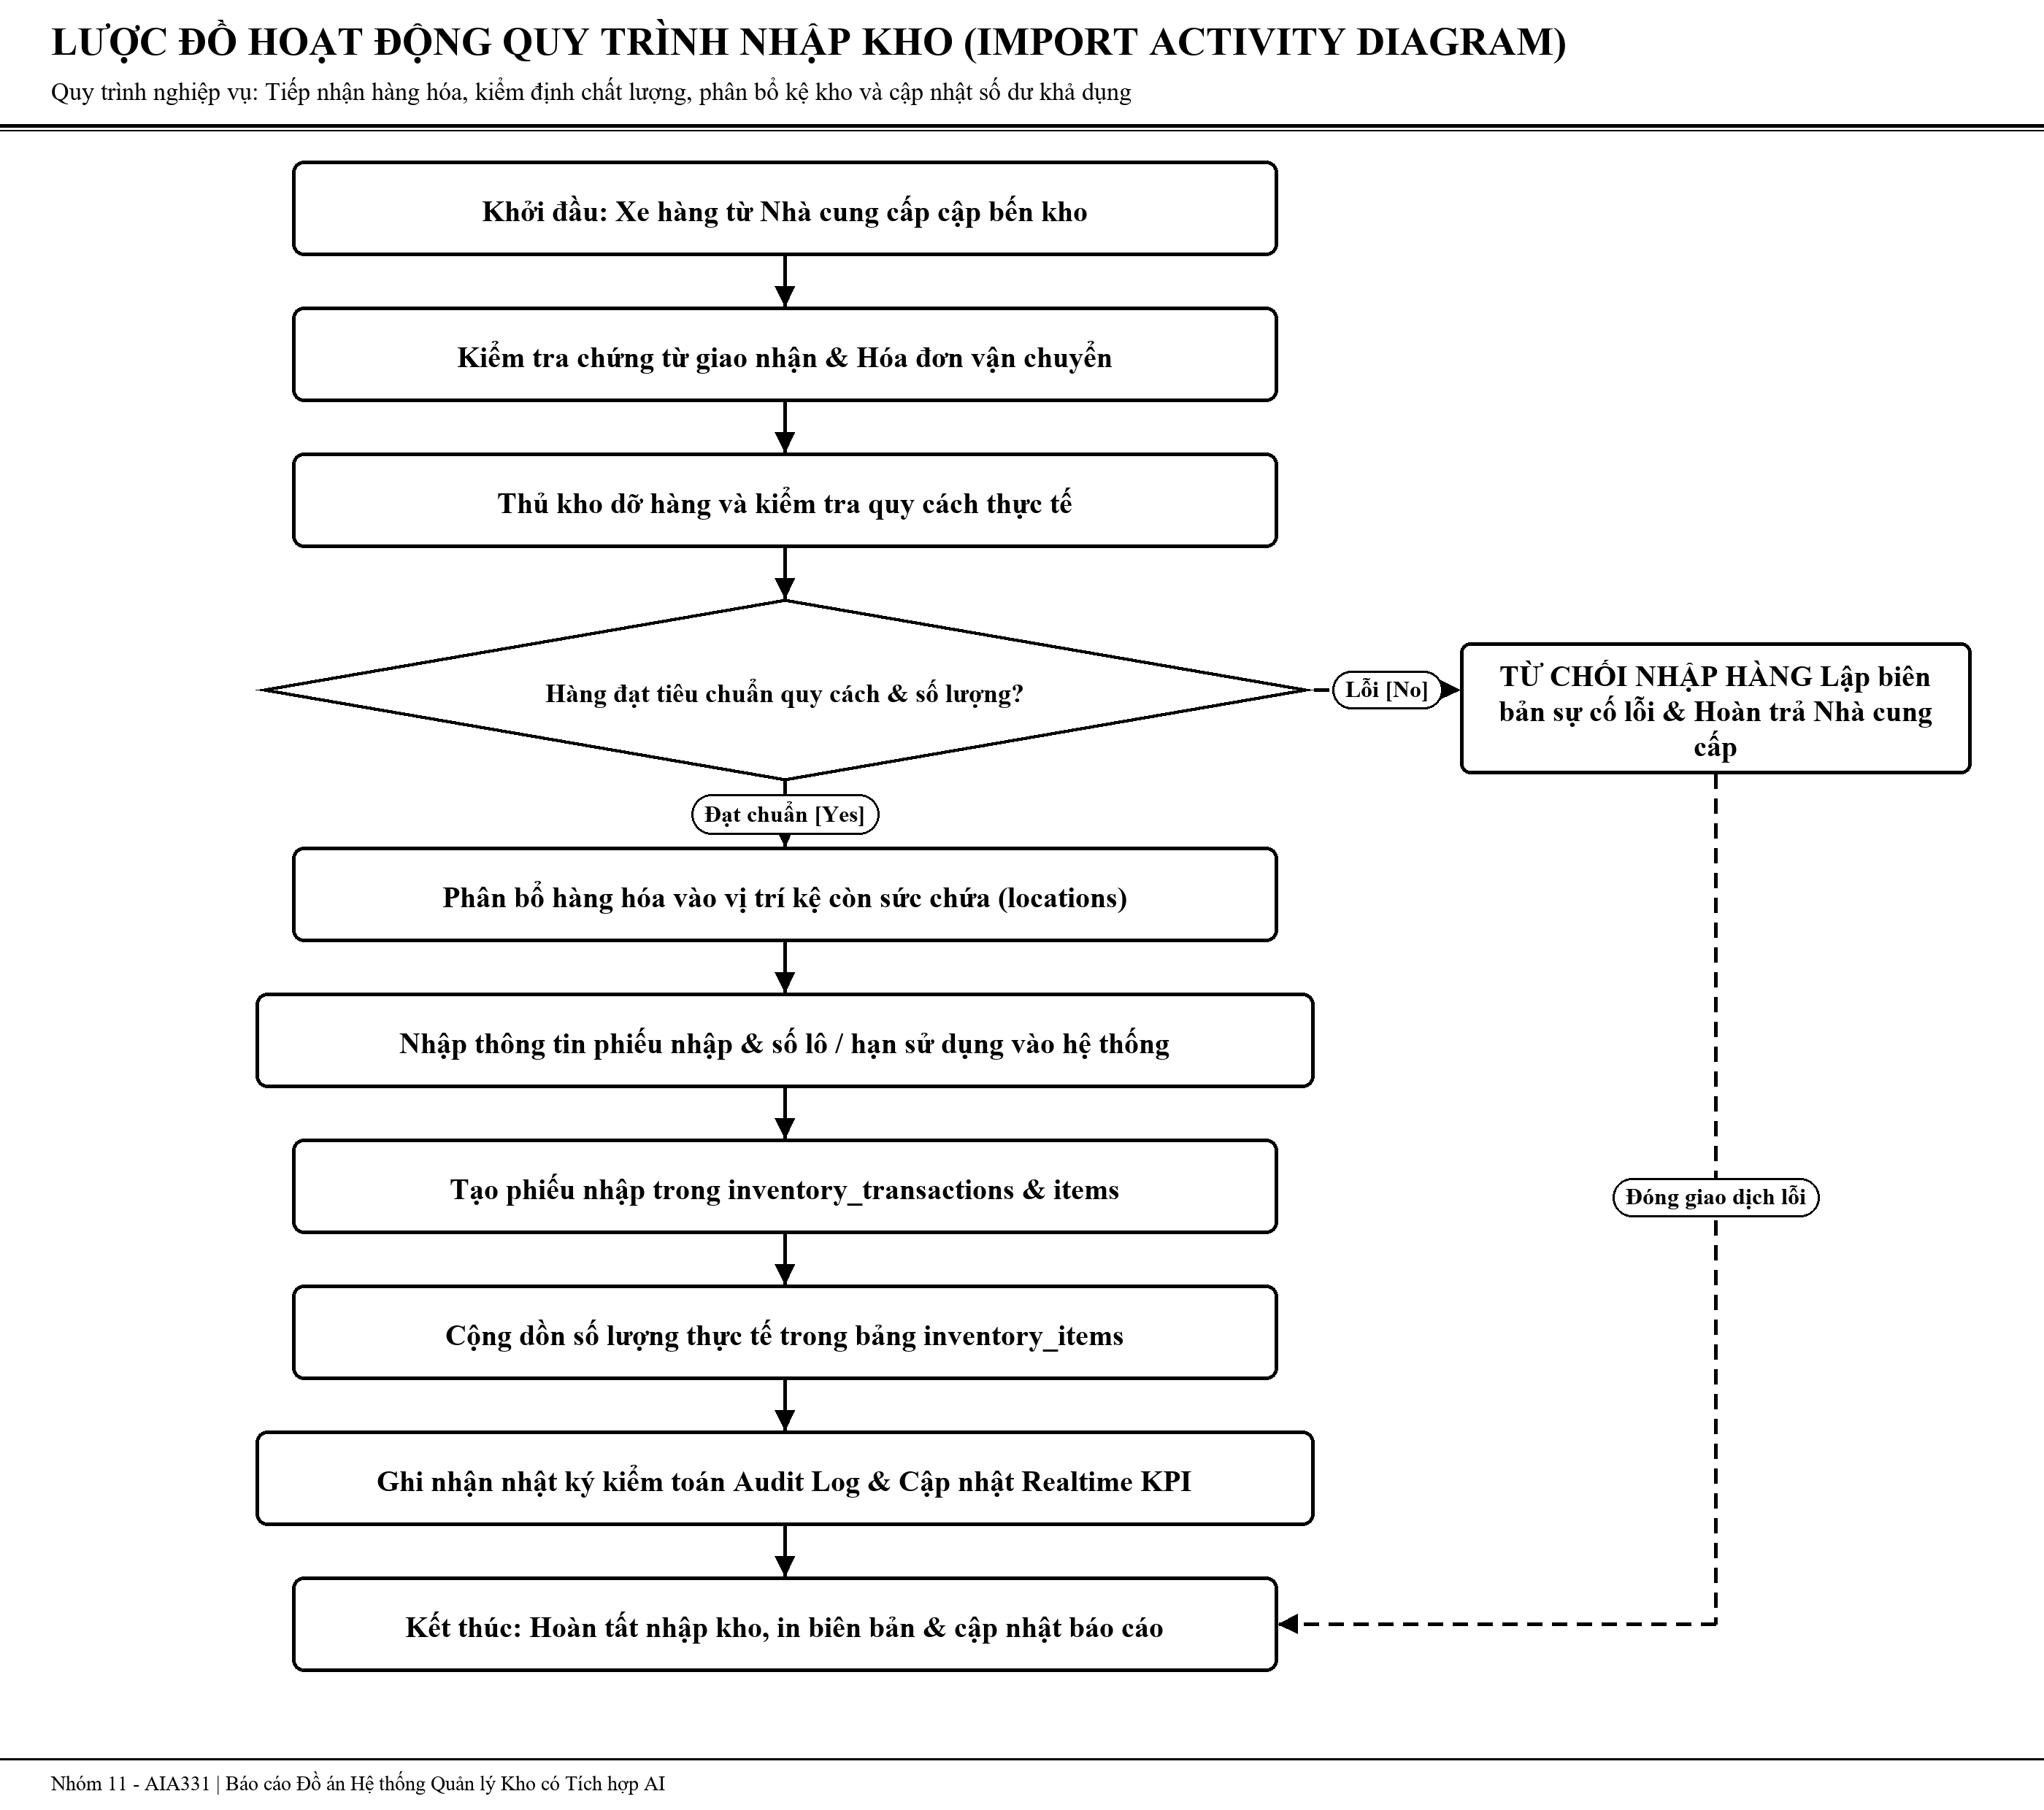
\includegraphics[width=0.85\textwidth]{04_luoc_do_hoat_dong_nhap_kho.png}
    \caption{Lược đồ hoạt động quy trình nghiệp vụ Nhập kho}
    \label{fig:act_import}
\end{figure}

\section{Lược đồ hoạt động quy trình Xuất kho}
Quy trình xuất kho kiểm tra số lượng tồn khả dụng để ngăn chặn xuất âm (Hình~\ref{fig:act_export}).

\begin{figure}[htbp]
    \centering
    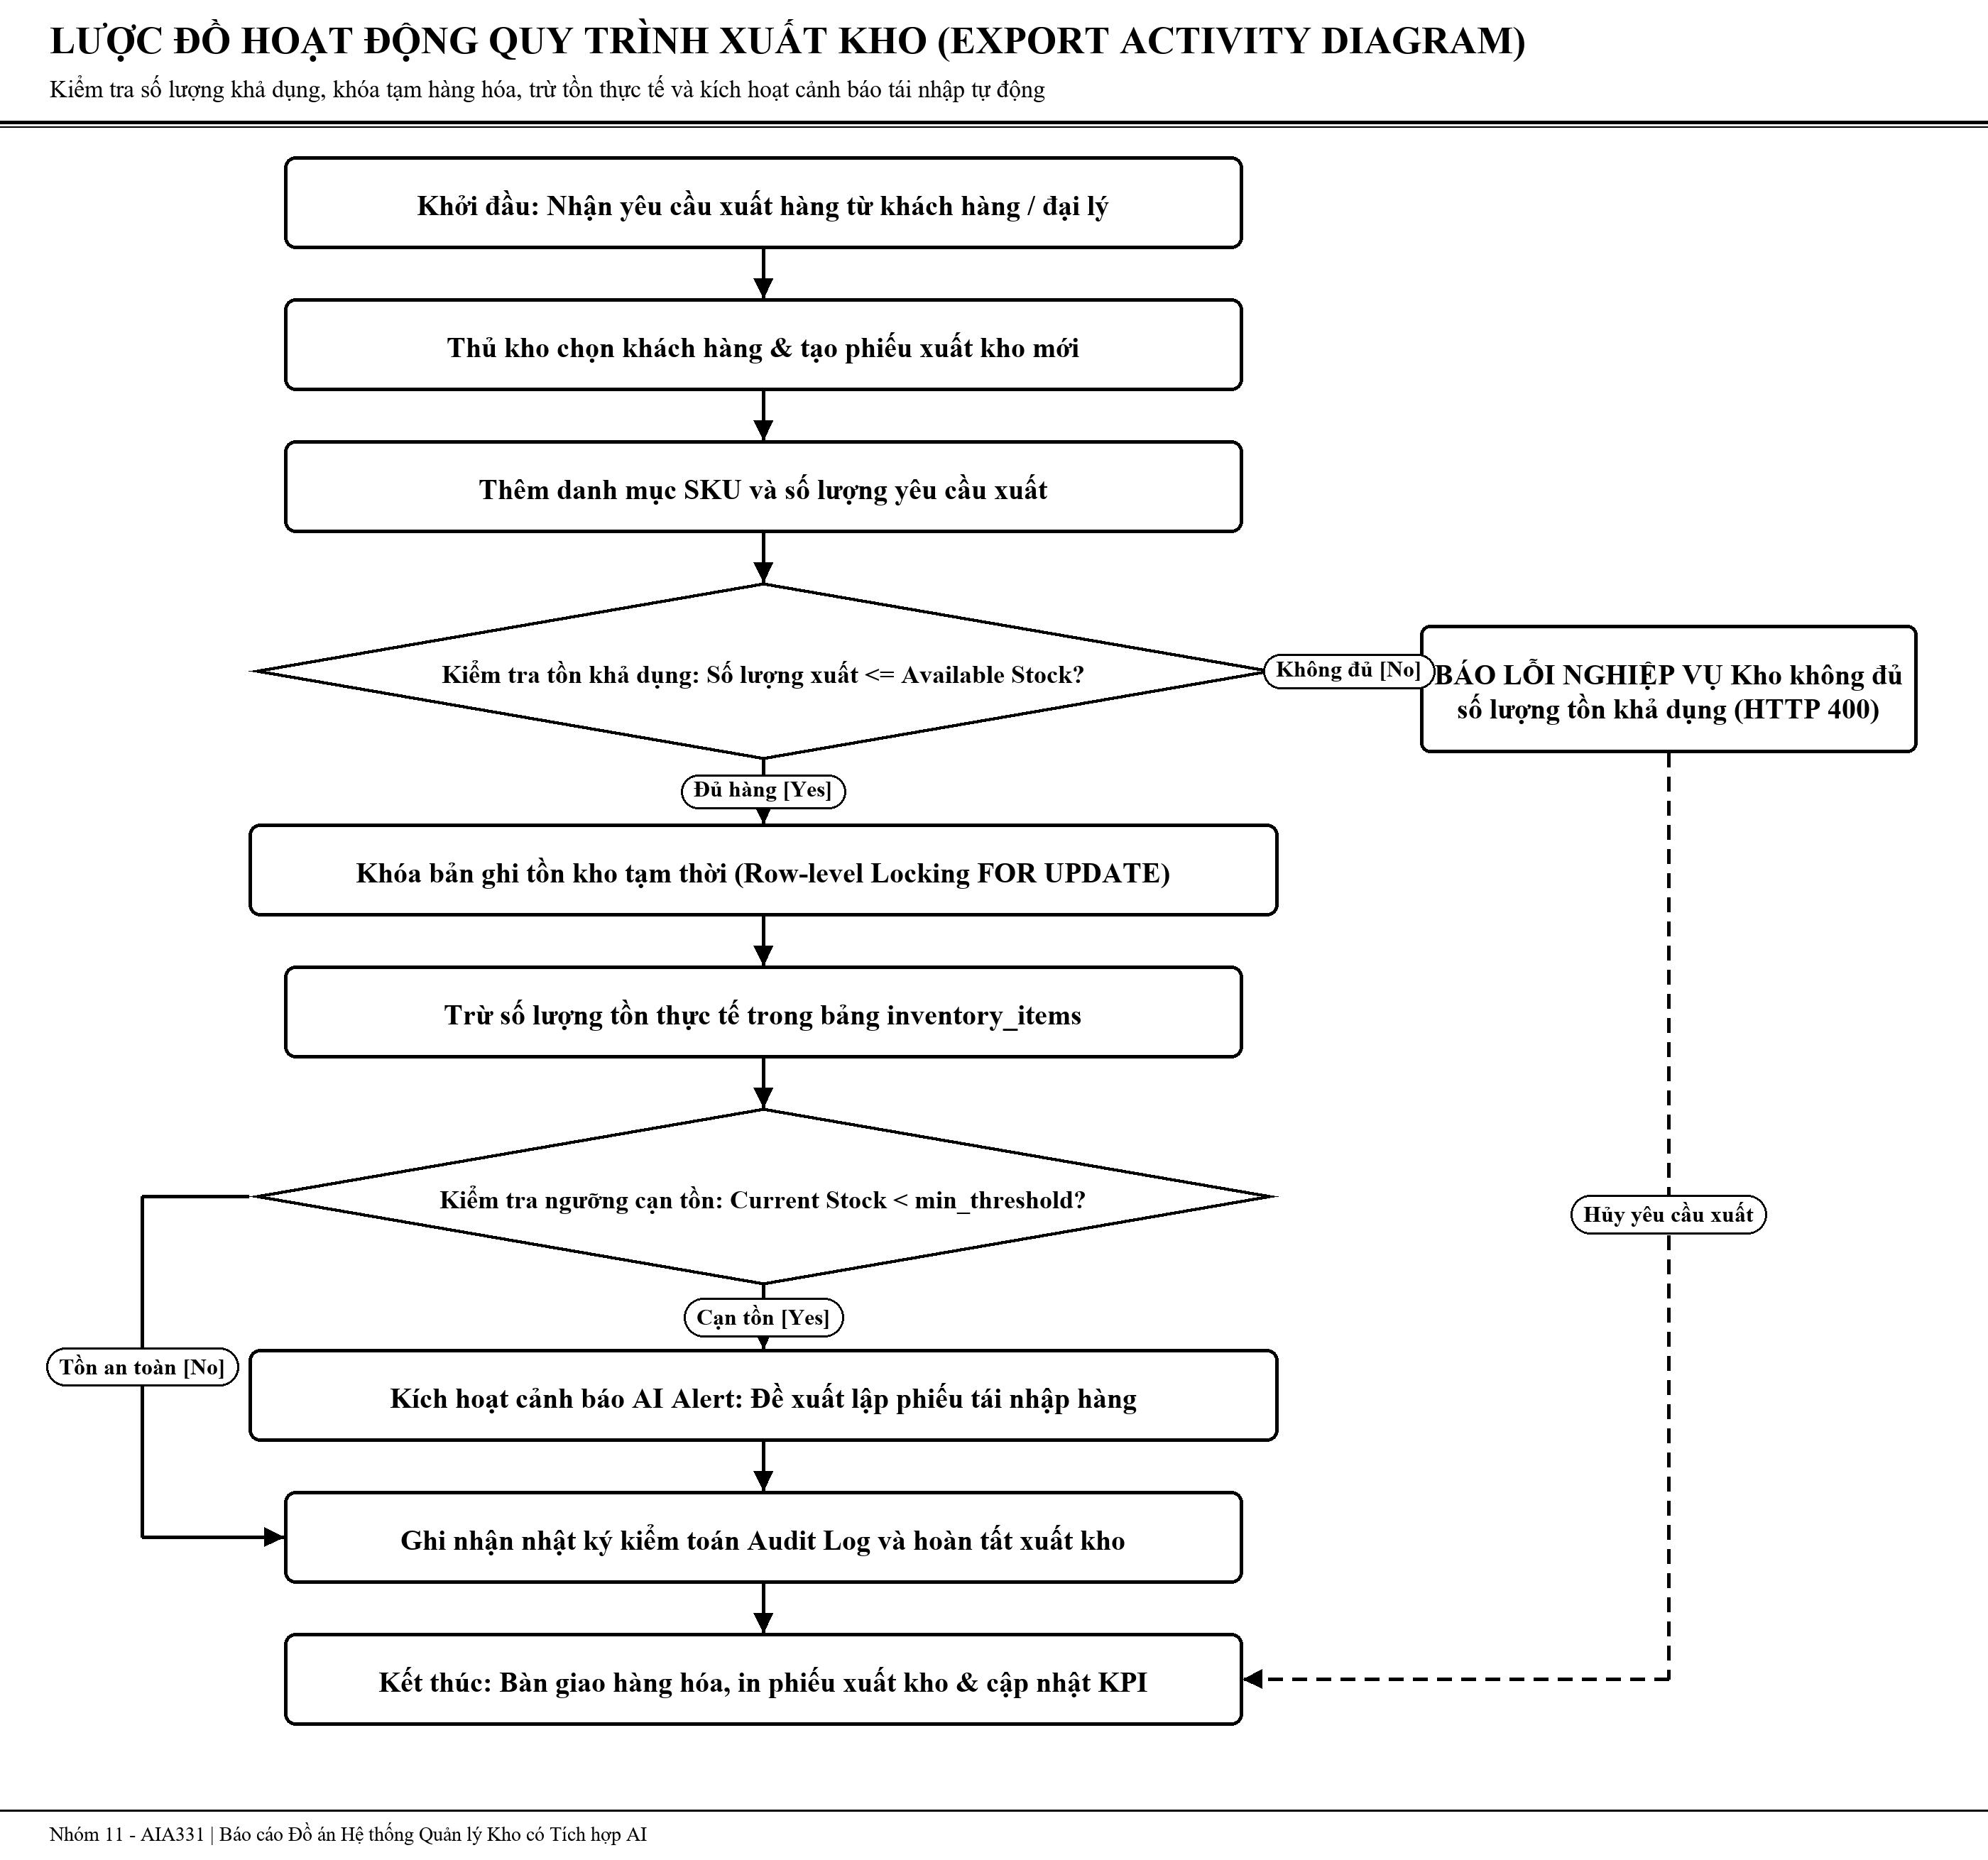
\includegraphics[width=0.85\textwidth]{05_luoc_do_hoat_dong_xuat_kho.png}
    \caption{Lược đồ hoạt động quy trình nghiệp vụ Xuất kho và kiểm tra tồn an toàn}
    \label{fig:act_export}
\end{figure}

\chapter{THIẾT KẾ CƠ SỞ DỮ LIỆU}
\label{ch:05}

\section{Sơ đồ thực thể liên kết (ERD) tổng quan 11 bảng chuẩn 3NF}
Cơ sở dữ liệu được thiết kế theo mô hình quan hệ RDBMS đạt chuẩn 3NF, loại bỏ tối đa dị thường dữ liệu (Hình~\ref{fig:erd}).

\begin{figure}[htbp]
    \centering
    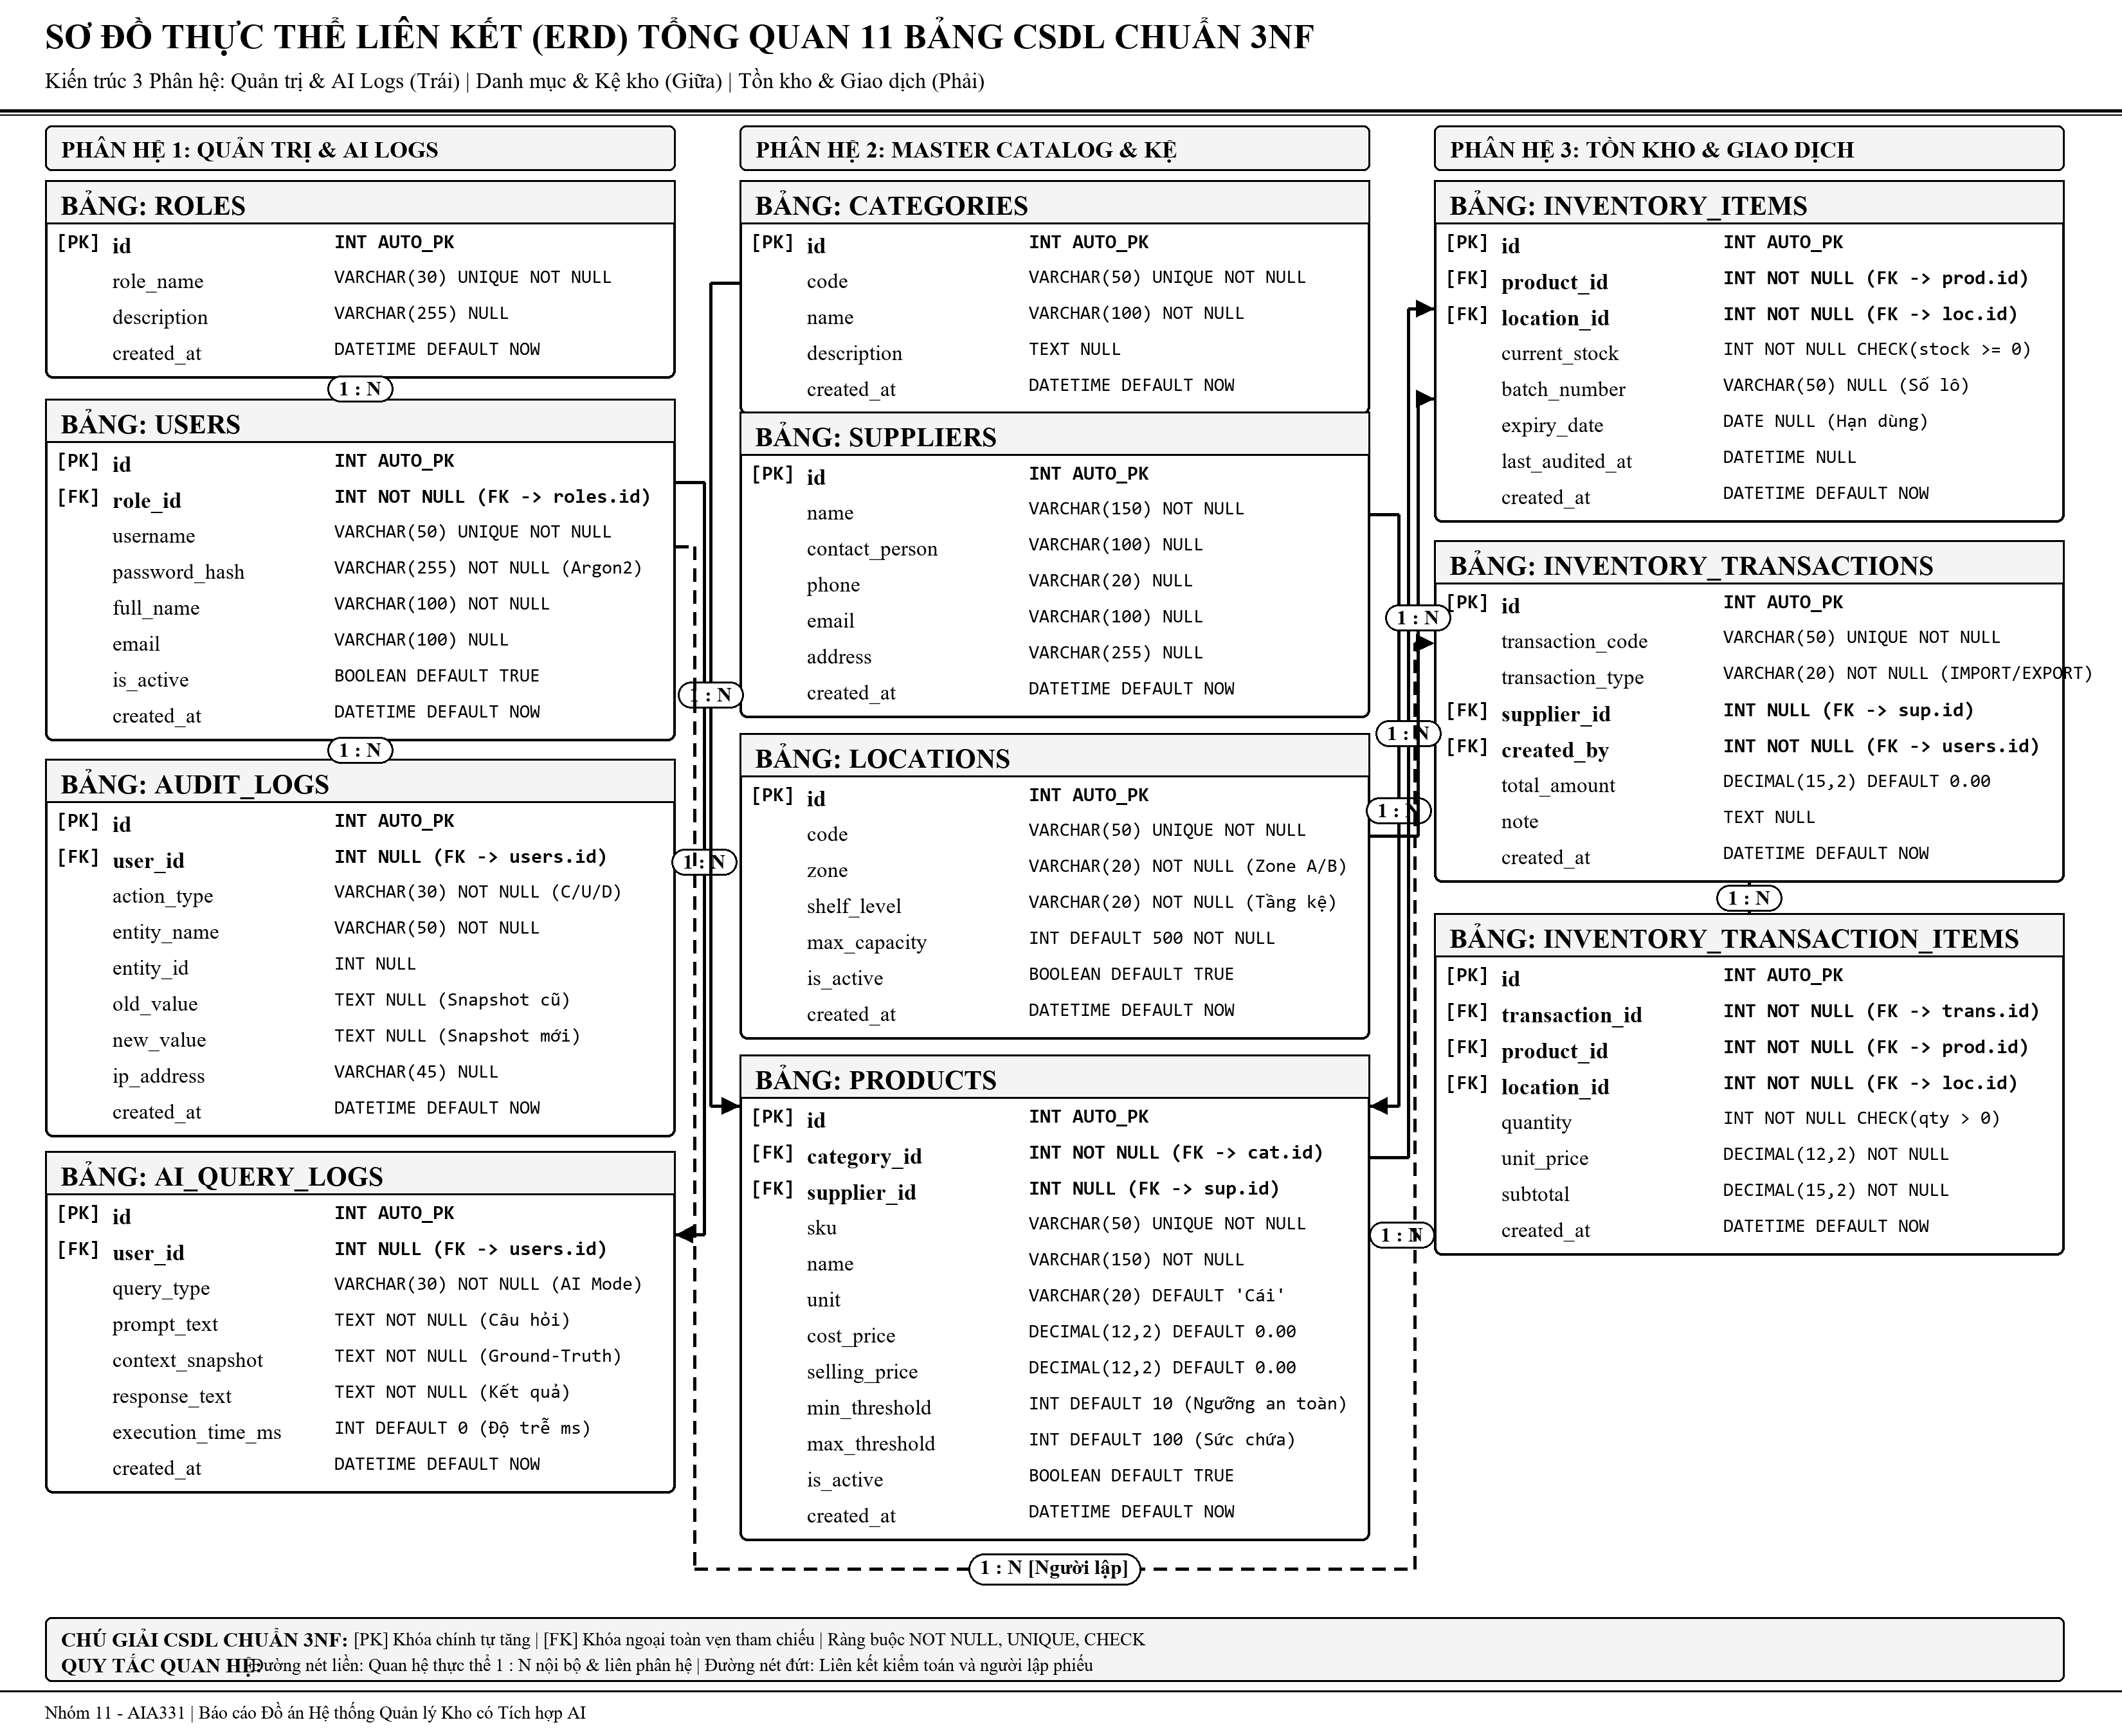
\includegraphics[width=0.98\textwidth]{03_so_do_erd_11_bang.png}
    \caption{Sơ đồ thực thể liên kết (ERD) tổng quan 11 bảng CSDL chuẩn 3NF (Nhóm 11)}
    \label{fig:erd}
\end{figure}

\section{Thiết kế chi tiết các phân hệ cơ sở dữ liệu}
Cấu trúc 11 bảng CSDL được phân rã chi tiết thành 3 phân hệ nghiệp vụ độc lập:

\subsection{Phân hệ Quản trị người dùng, Phân quyền RBAC và AI Logs}
Quản lý vai trò phân quyền, tài khoản mật khẩu băm Argon2, vết kiểm toán Audit Trail và nhật ký prompt AI (Hình~\ref{fig:erd_users_ai}).
\begin{figure}[htbp]
    \centering
    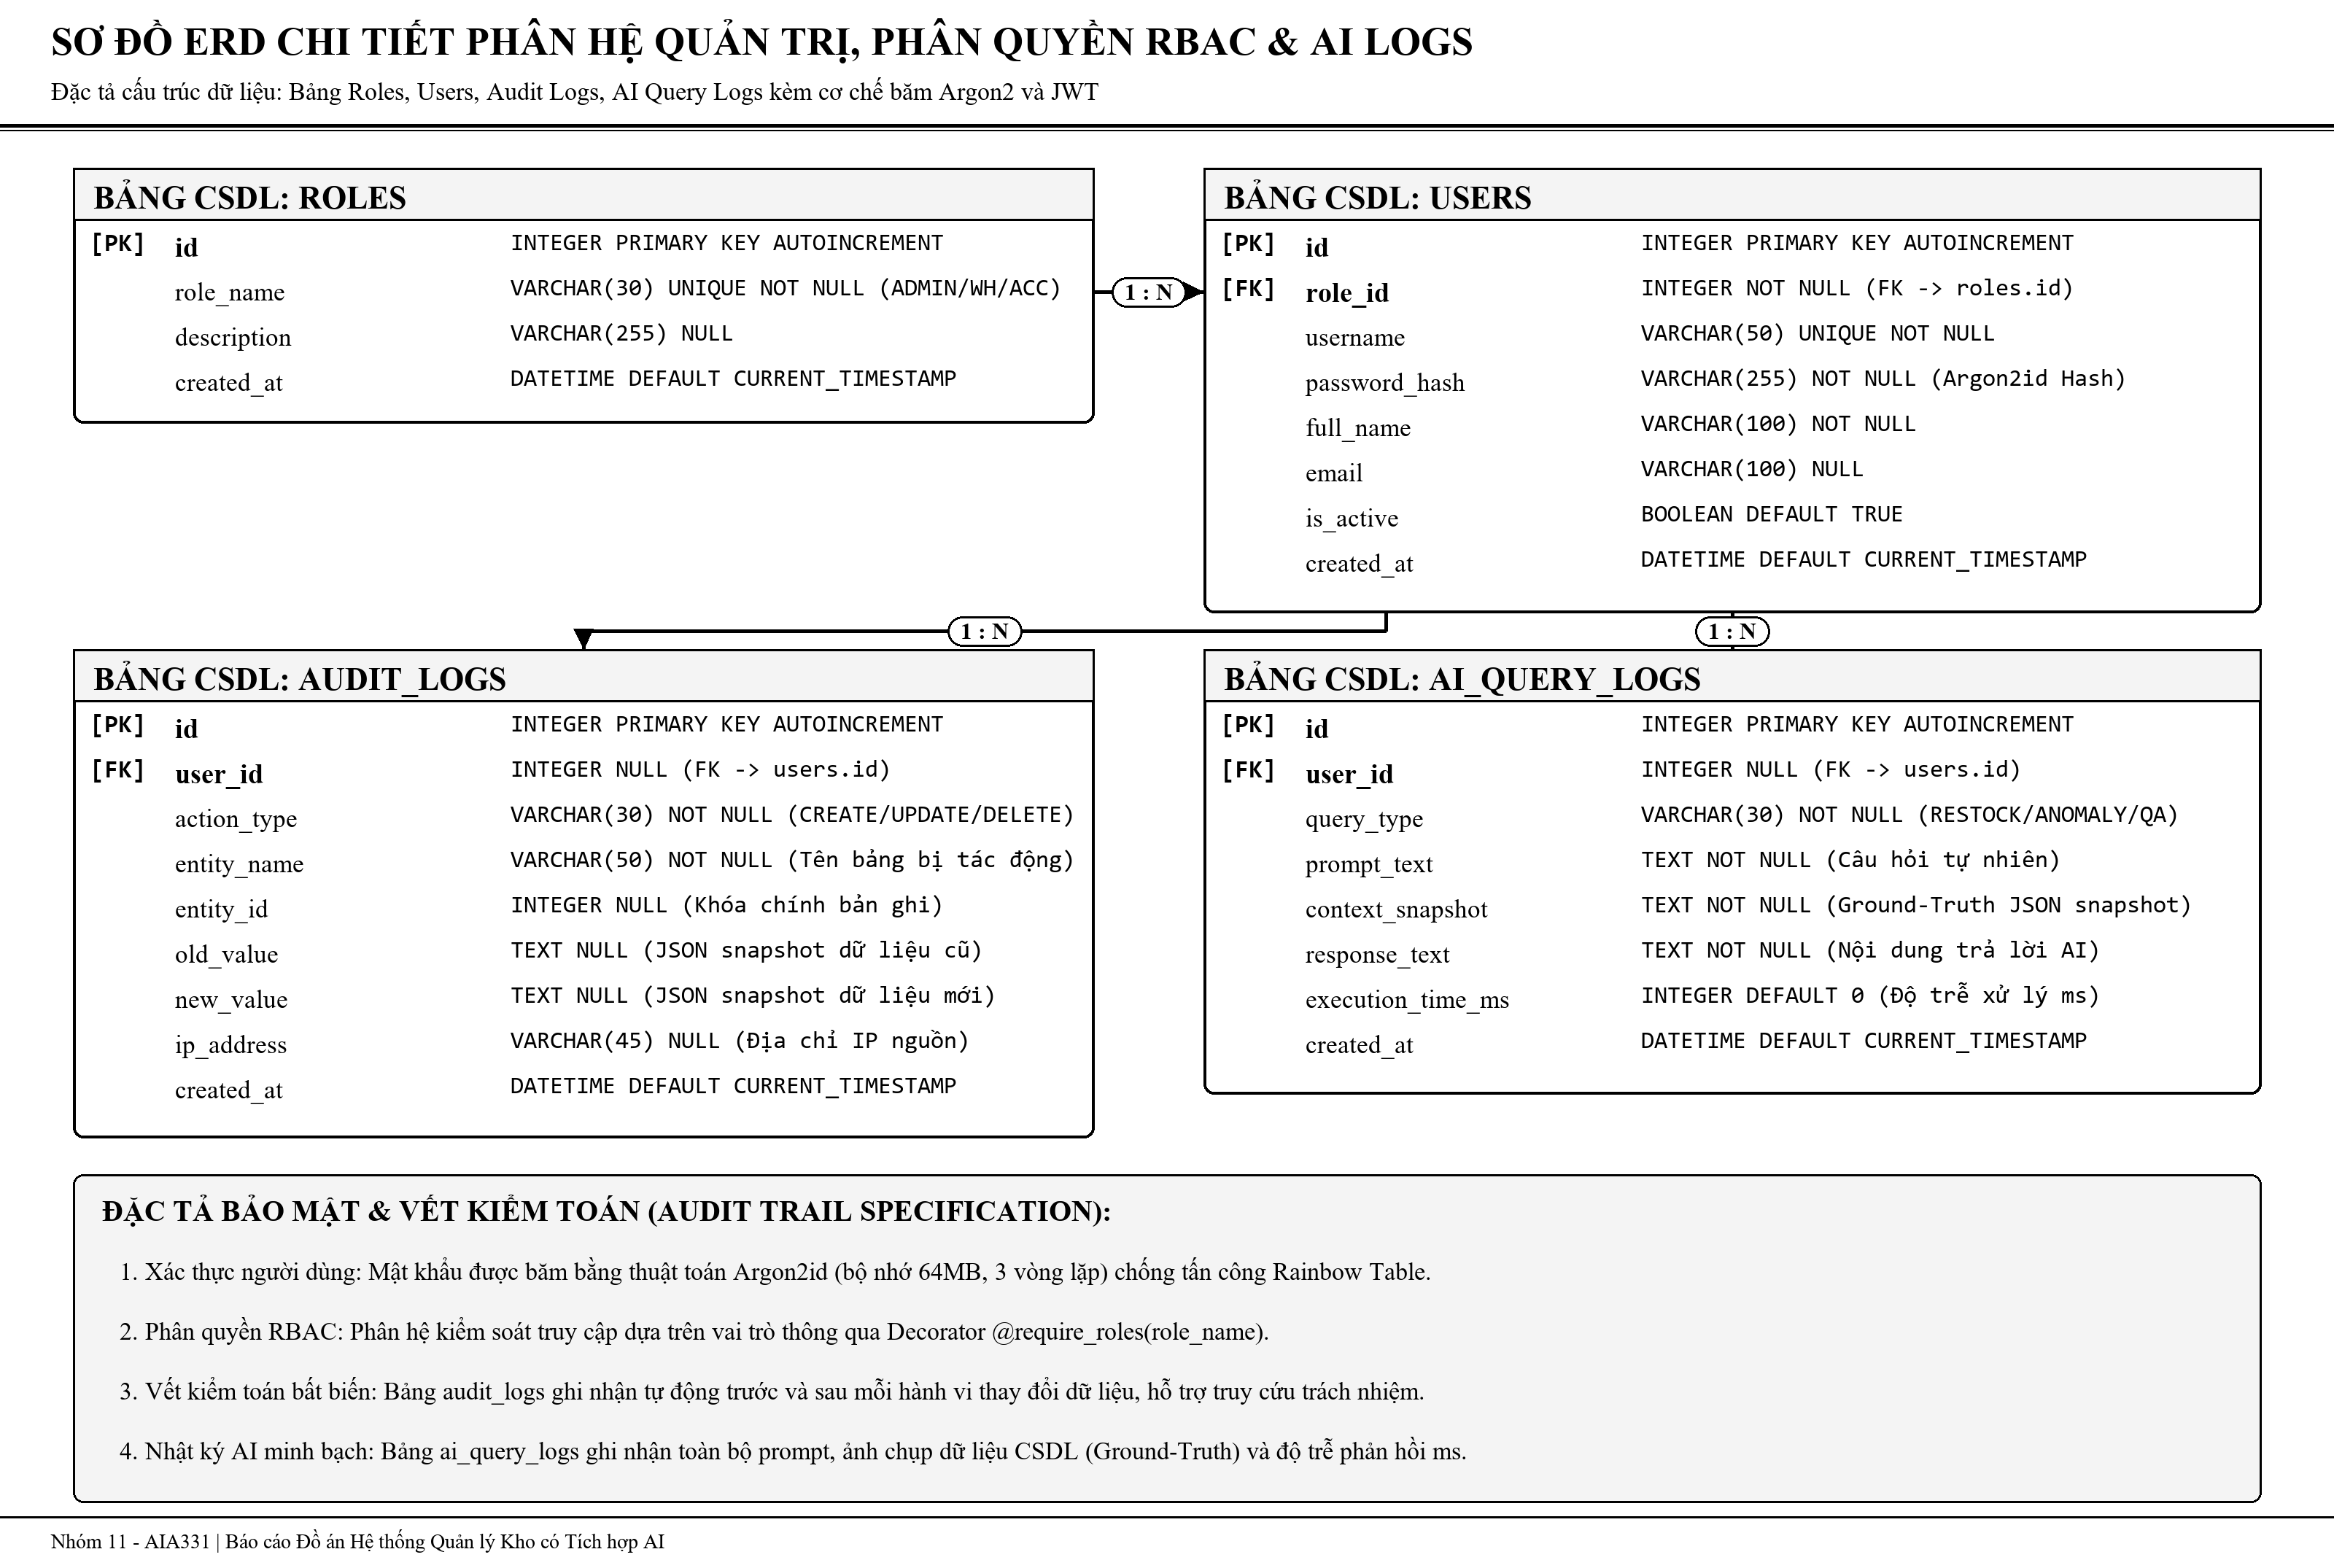
\includegraphics[width=0.95\textwidth]{03a_erd_nhom_nguoi_dung_ai.png}
    \caption{Sơ đồ ERD chi tiết phân hệ Quản trị người dùng, Phân quyền RBAC và AI Logs (Nhóm 11)}
    \label{fig:erd_users_ai}
\end{figure}

\subsection{Phân hệ Danh mục Hàng hóa, Nhà cung cấp và Vị trí Kệ kho}
Quản lý danh mục hàng hóa, nhà cung cấp, mã vị trí vật lý theo cấu trúc Zone-Shelf-Level và mã SKU duy nhất (Hình~\ref{fig:erd_master}).
\begin{figure}[htbp]
    \centering
    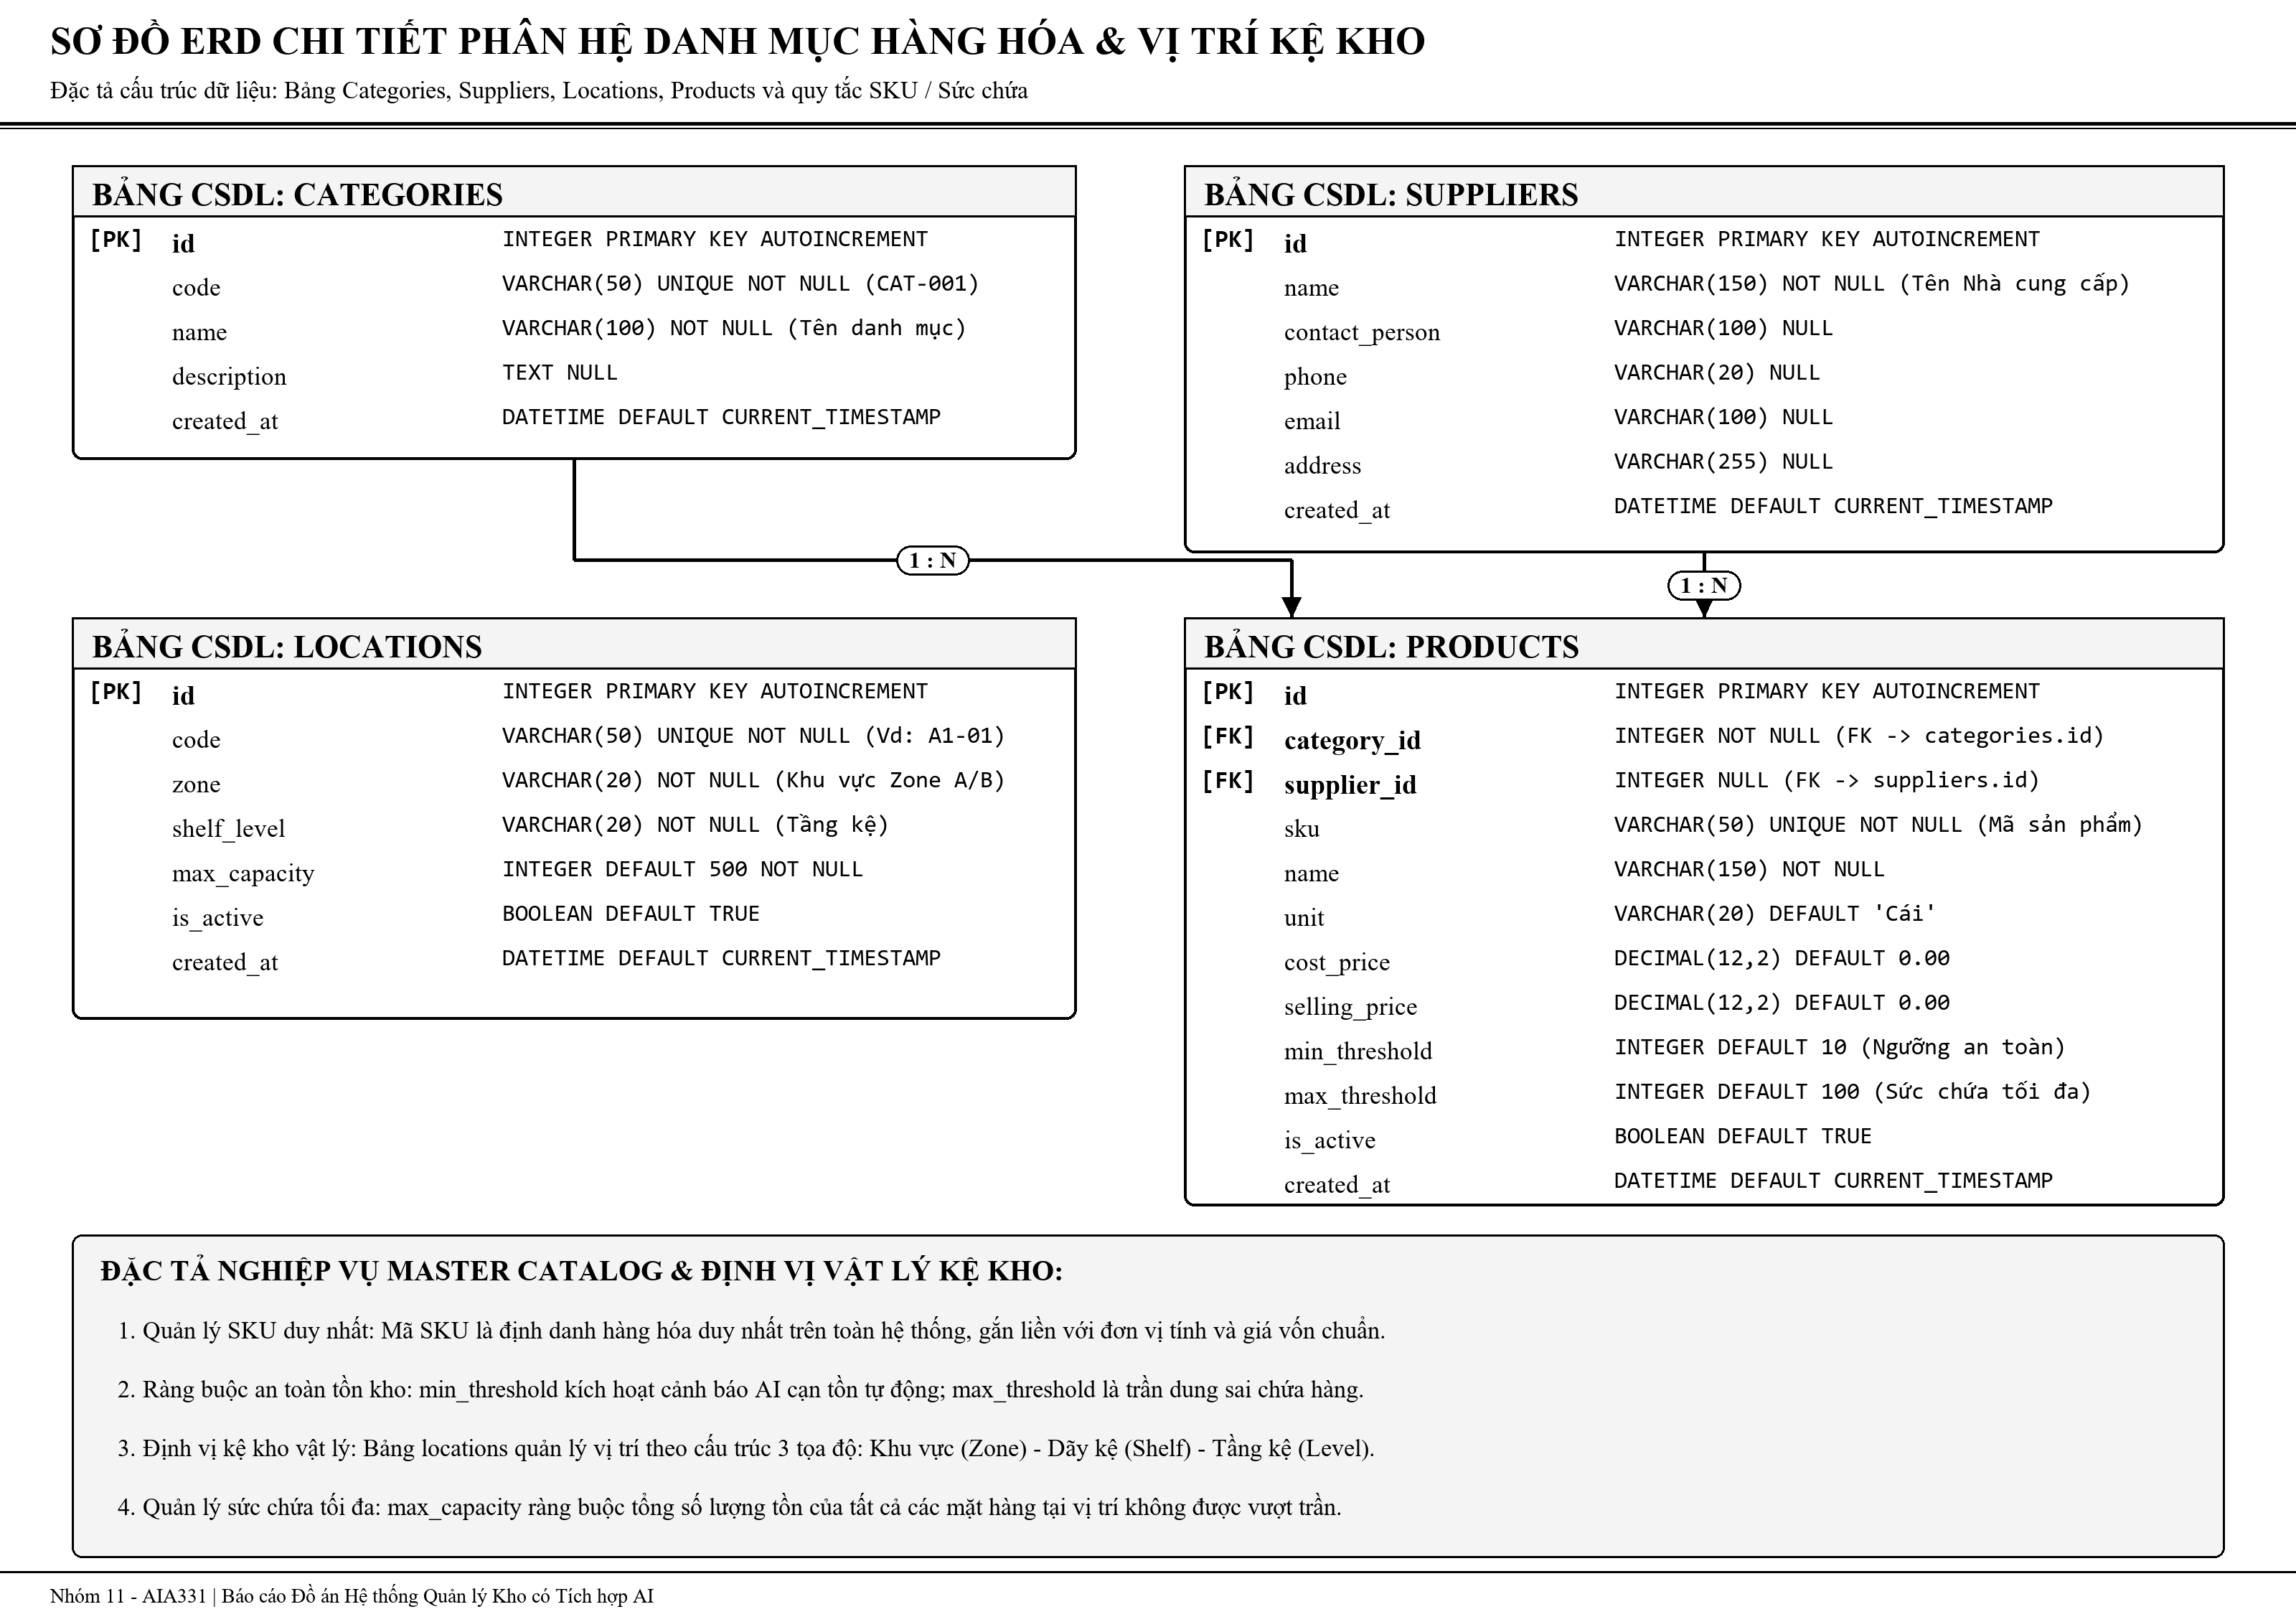
\includegraphics[width=0.95\textwidth]{03b_erd_nhom_danh_muc_kho.png}
    \caption{Sơ đồ ERD chi tiết phân hệ Danh mục Hàng hóa, Nhà cung cấp và Vị trí Kệ kho (Nhóm 11)}
    \label{fig:erd_master}
\end{figure}

\subsection{Phân hệ Quản lý Tồn kho Khả dụng và Giao dịch Xuất Nhập kho}
Quản lý số lượng tồn thực tế, số lô sản xuất, hạn sử dụng và chi tiết phiếu giao dịch có khóa dòng an toàn (Hình~\ref{fig:erd_trans}).
\begin{figure}[htbp]
    \centering
    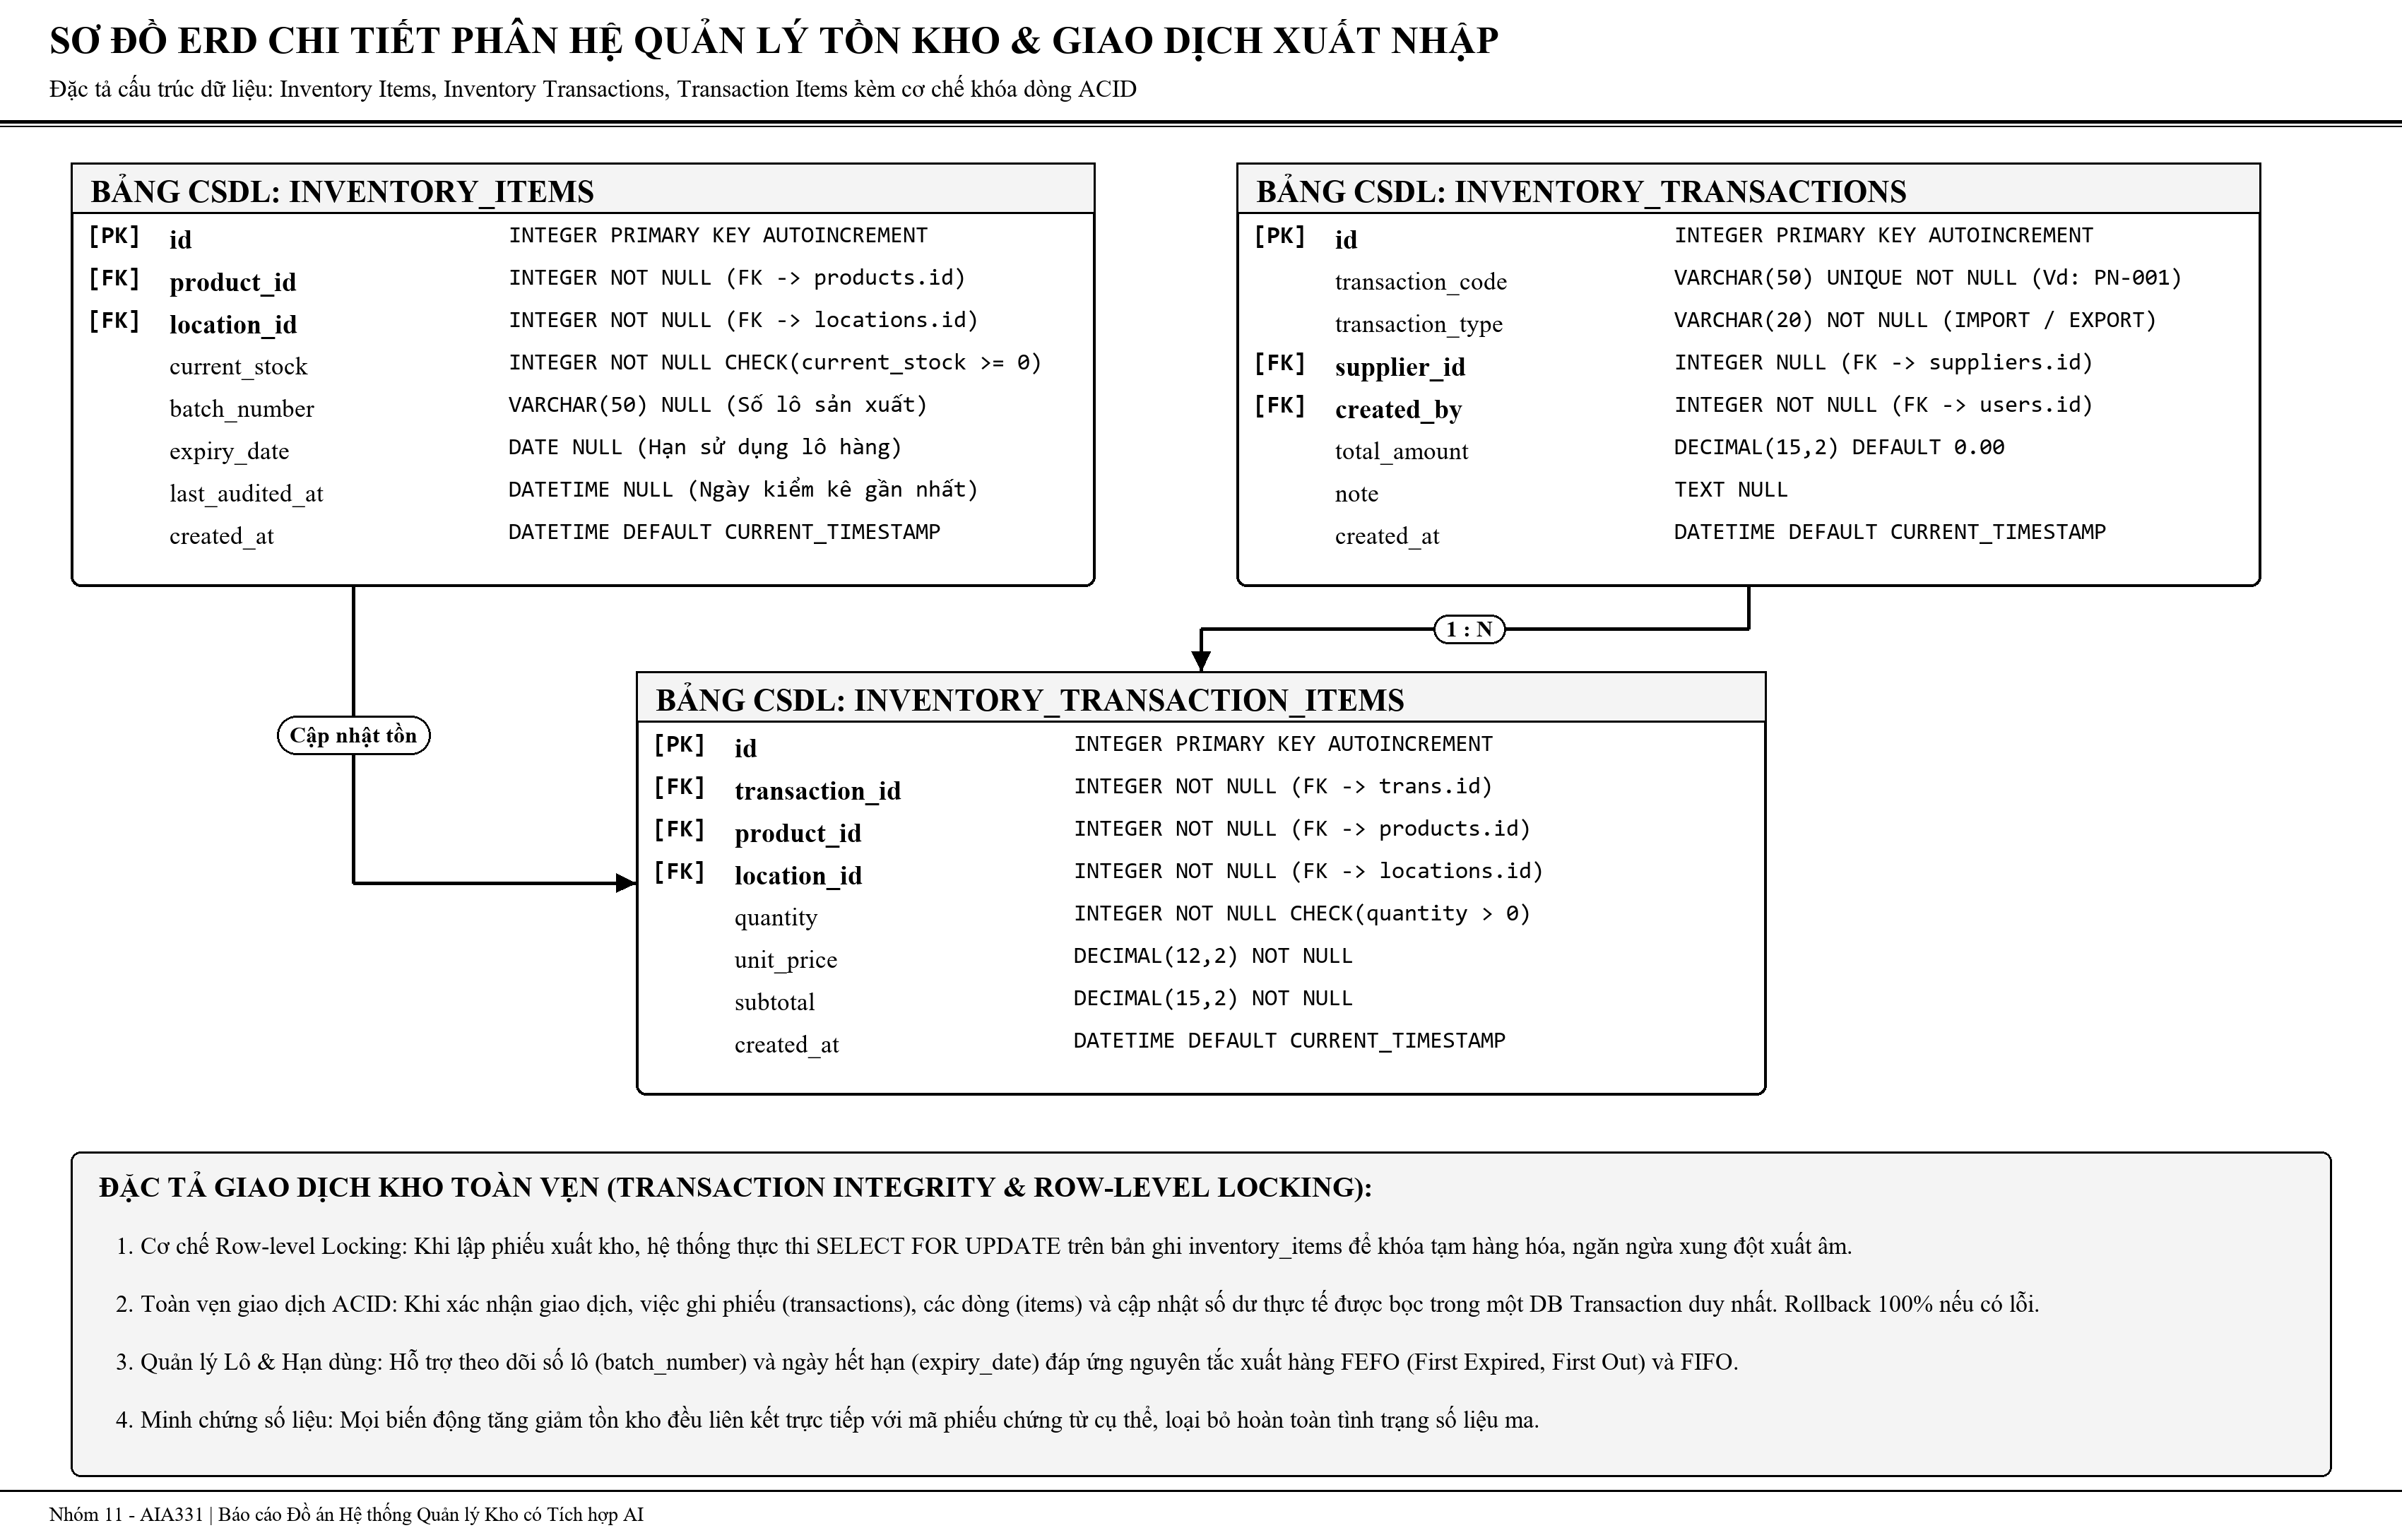
\includegraphics[width=0.95\textwidth]{03c_erd_nhom_ton_kho_giao_dich.png}
    \caption{Sơ đồ ERD chi tiết phân hệ Quản lý Tồn kho Khả dụng và Giao dịch Xuất Nhập kho (Nhóm 11)}
    \label{fig:erd_trans}
\end{figure}

\section{Danh mục 11 bảng cơ sở dữ liệu quan hệ}
Bao gồm: \texttt{roles}, \texttt{users}, \texttt{categories}, \texttt{suppliers}, \texttt{locations}, \texttt{products}, \texttt{inventory\_items}, \texttt{inventory\_transactions}, \texttt{inventory\_transaction\_items}, \texttt{audit\_logs}, \texttt{ai\_query\_logs}.

\chapter{KIẾN TRÚC HỆ THỐNG}
\label{ch:06}

\section{Thiết kế Kiến trúc 3 tầng tổng thể}
Hệ thống tuân thủ mô hình Kiến trúc 3 tầng phân tách độc lập các trách nhiệm (Hình~\ref{fig:arch}):
\begin{figure}[htbp]
    \centering
    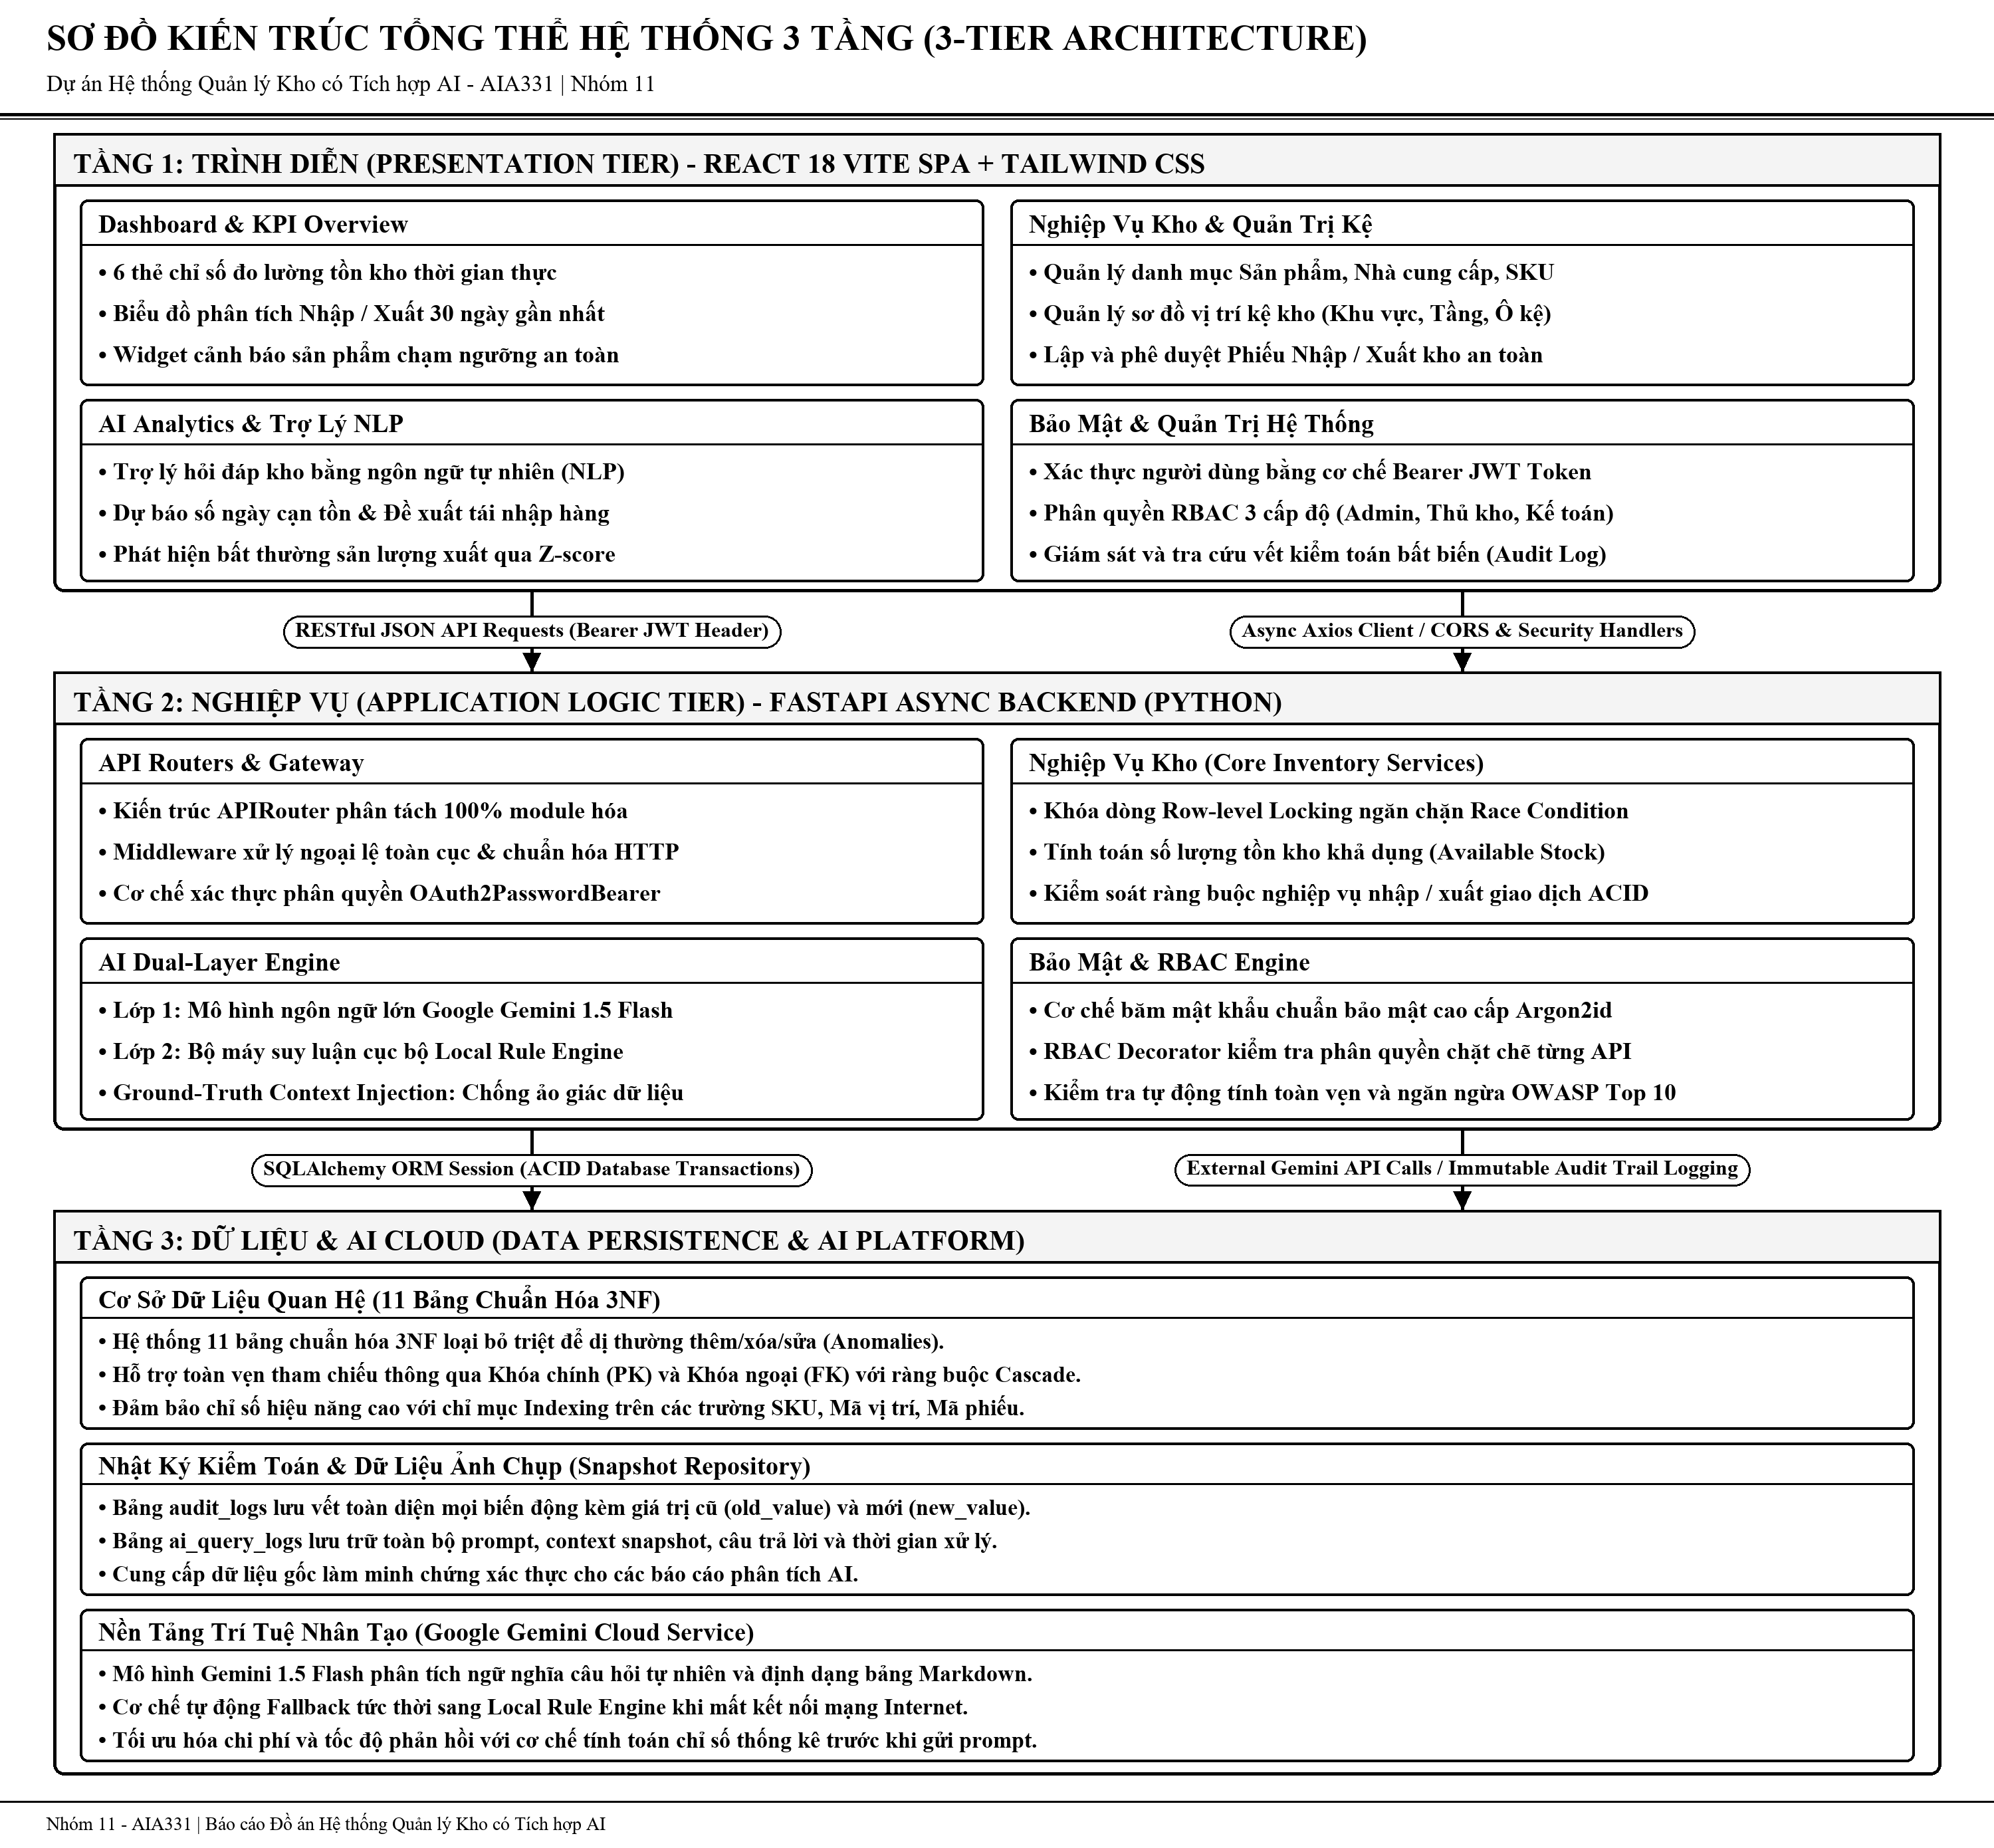
\includegraphics[width=0.95\textwidth]{01_so_do_kien_truc_he_thong.png}
    \caption{Sơ đồ Kiến trúc tổng thể 3 tầng hệ thống Quản lý Kho AI (Nhóm 11)}
    \label{fig:arch}
\end{figure}

\section{Sơ đồ tuần tự xử lý giao dịch an toàn}
Hình~\ref{fig:seq_trans} thể hiện sơ đồ tuần tự giao dịch nhập xuất kho an toàn có khóa dòng và ghi vết kiểm toán.
\begin{figure}[htbp]
    \centering
    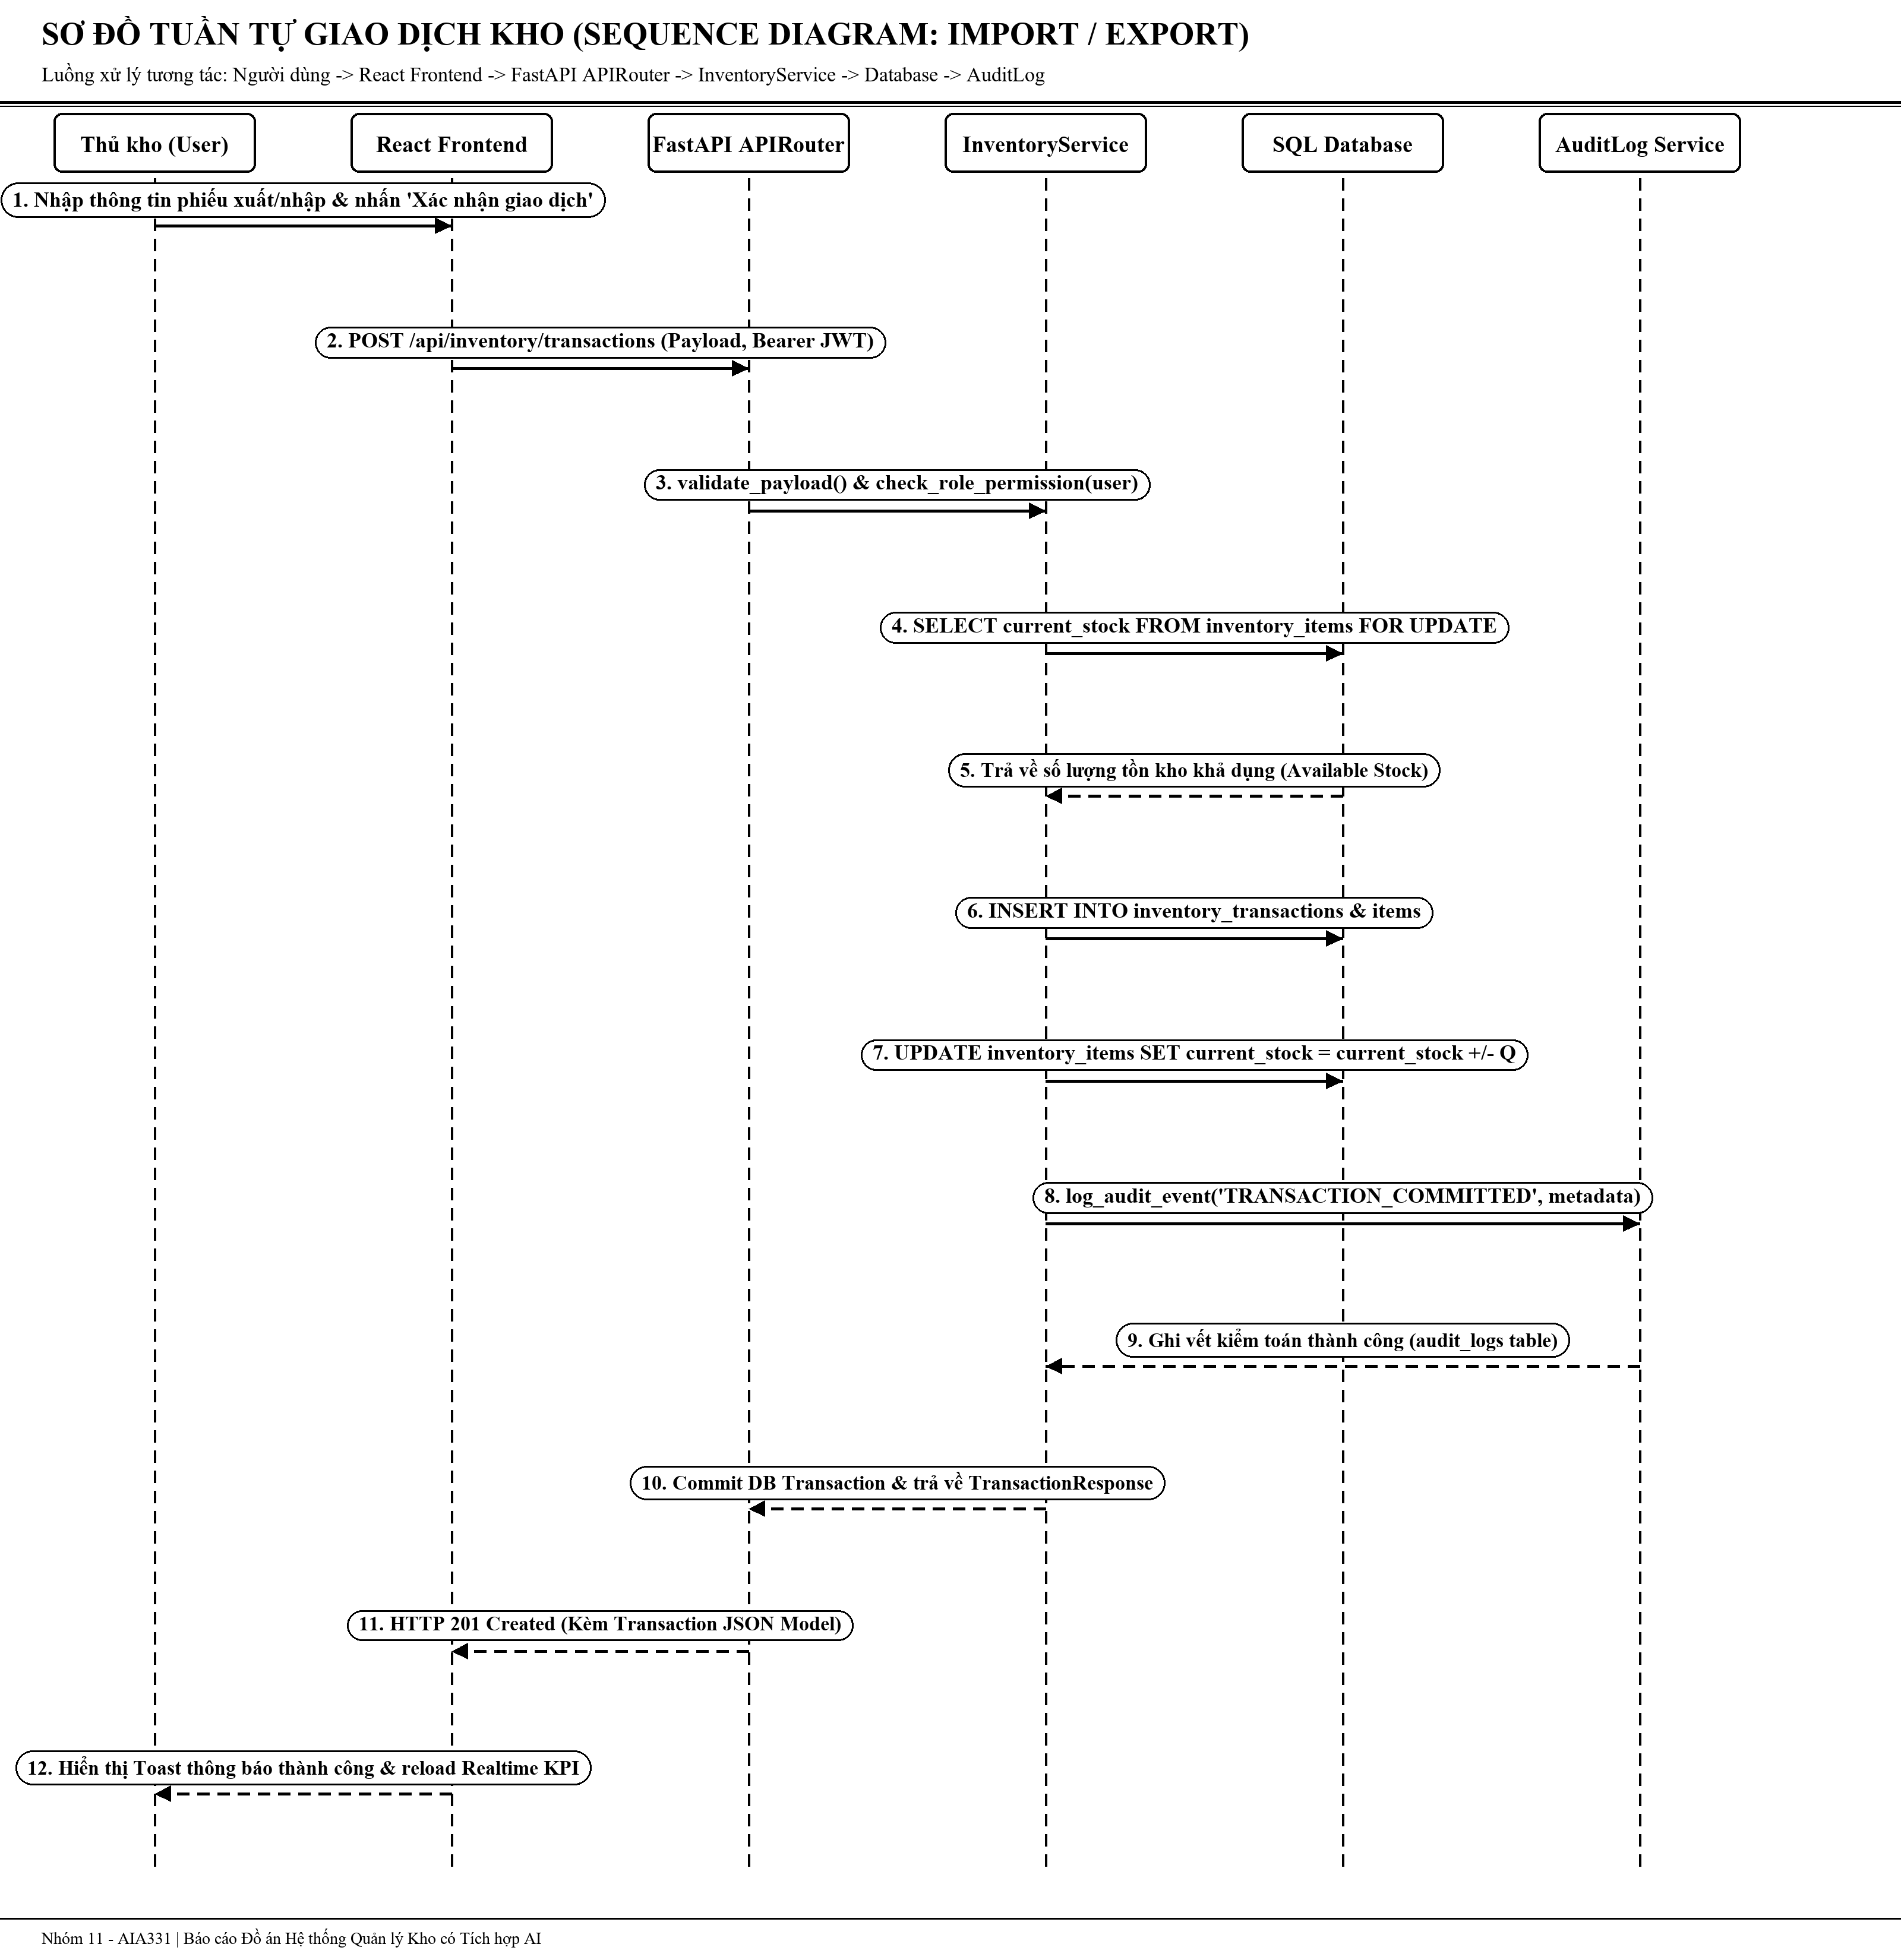
\includegraphics[width=0.92\textwidth]{06_so_do_tuan_tu_nhap_xuat.png}
    \caption{Sơ đồ tuần tự xử lý giao dịch kho an toàn}
    \label{fig:seq_trans}
\end{figure}

\section{Sơ đồ điều hướng giao diện người dùng}
Hình~\ref{fig:sitemap} mô tả cấu trúc điều hướng Sitemap giao diện người dùng SaaS UI.
\begin{figure}[htbp]
    \centering
    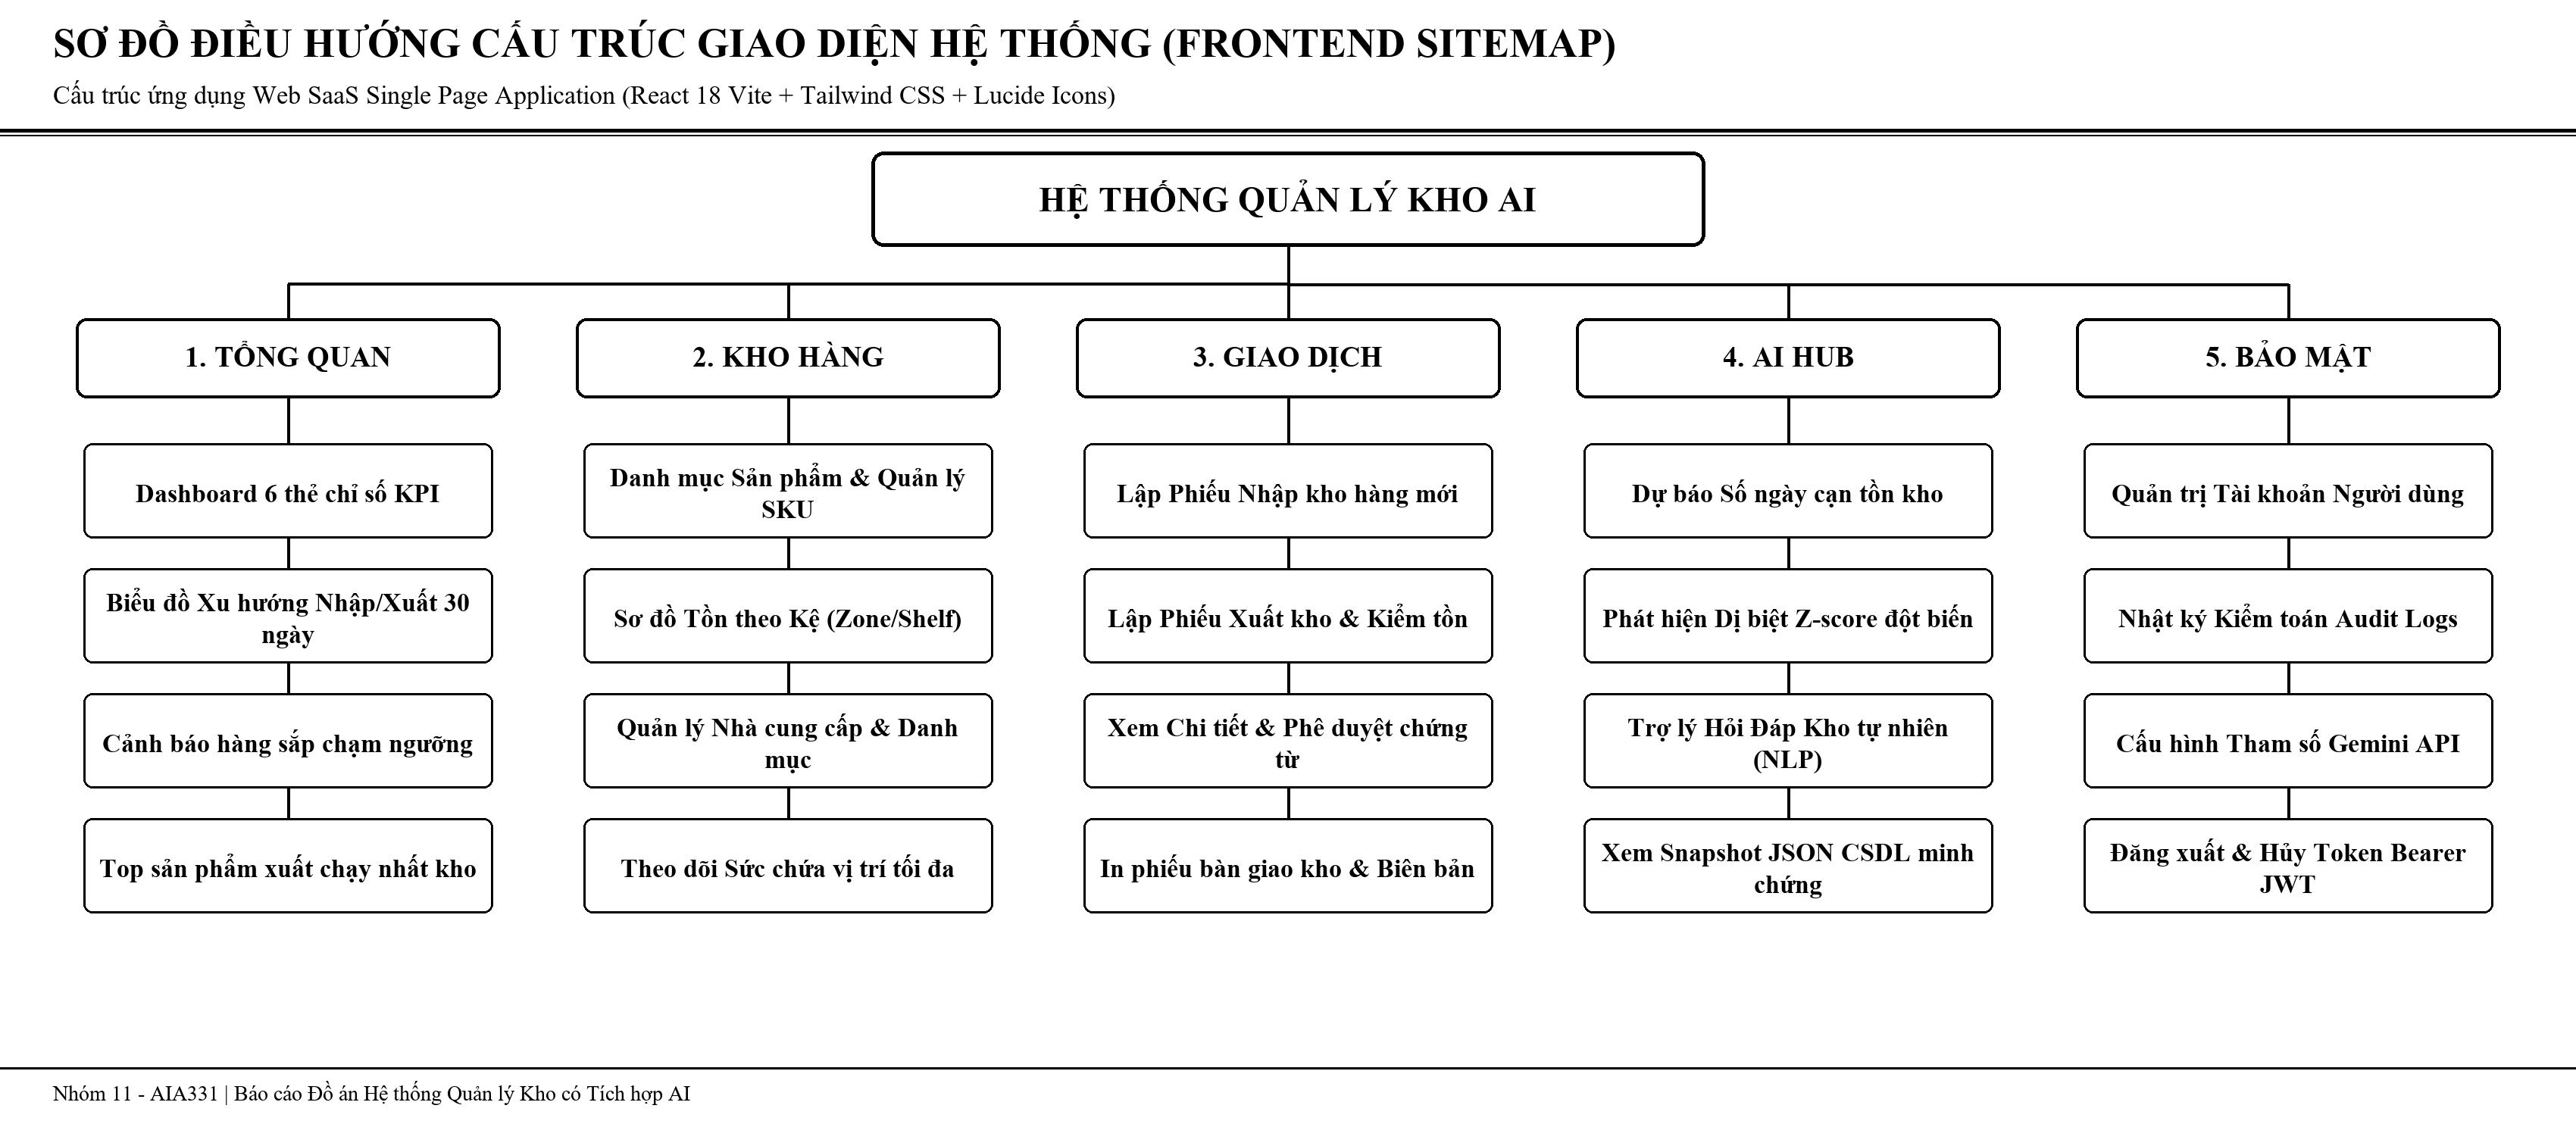
\includegraphics[width=0.92\textwidth]{10_so_do_sitemap_giao_dien.png}
    \caption{Sơ đồ cấu trúc điều hướng phân hệ giao diện người dùng (Sitemap)}
    \label{fig:sitemap}
\end{figure}

\chapter{THIẾT KẾ CHI TIẾT CHỨC NĂNG}
\label{ch:07}

\section{Phân hệ Quản lý Sản phẩm và SKU}
Hỗ trợ CRUD danh mục sản phẩm, mã SKU, thiết lập giá vốn, giá bán lẻ và định mức an toàn tối thiểu/tối đa.

\section{Phân hệ Giao dịch Nhập xuất kho}
Tự động tính toán tổng tiền, kiểm tra tồn khả dụng, phân bổ vị trí ô kệ và cập nhật số lượng tồn theo thời gian thực.

\section{Phân hệ Dashboard và Báo cáo tài chính kho}
Hiển thị 6 chỉ số KPI kho: Tổng số sản phẩm, tổng tồn kho, số mặt hàng sắp hết, giá trị tồn kho theo VNĐ, doanh thu và chi phí.

\chapter{THIẾT KẾ VÀ TÍCH HỢP AI}
\label{ch:08}

\section{Kiến trúc Pipeline AI 2 lớp (Dual-layer Resilience)}
Hệ thống tích hợp Pipeline AI 2 lớp linh hoạt (Hình~\ref{fig:ai_pipe}):
\begin{figure}[htbp]
    \centering
    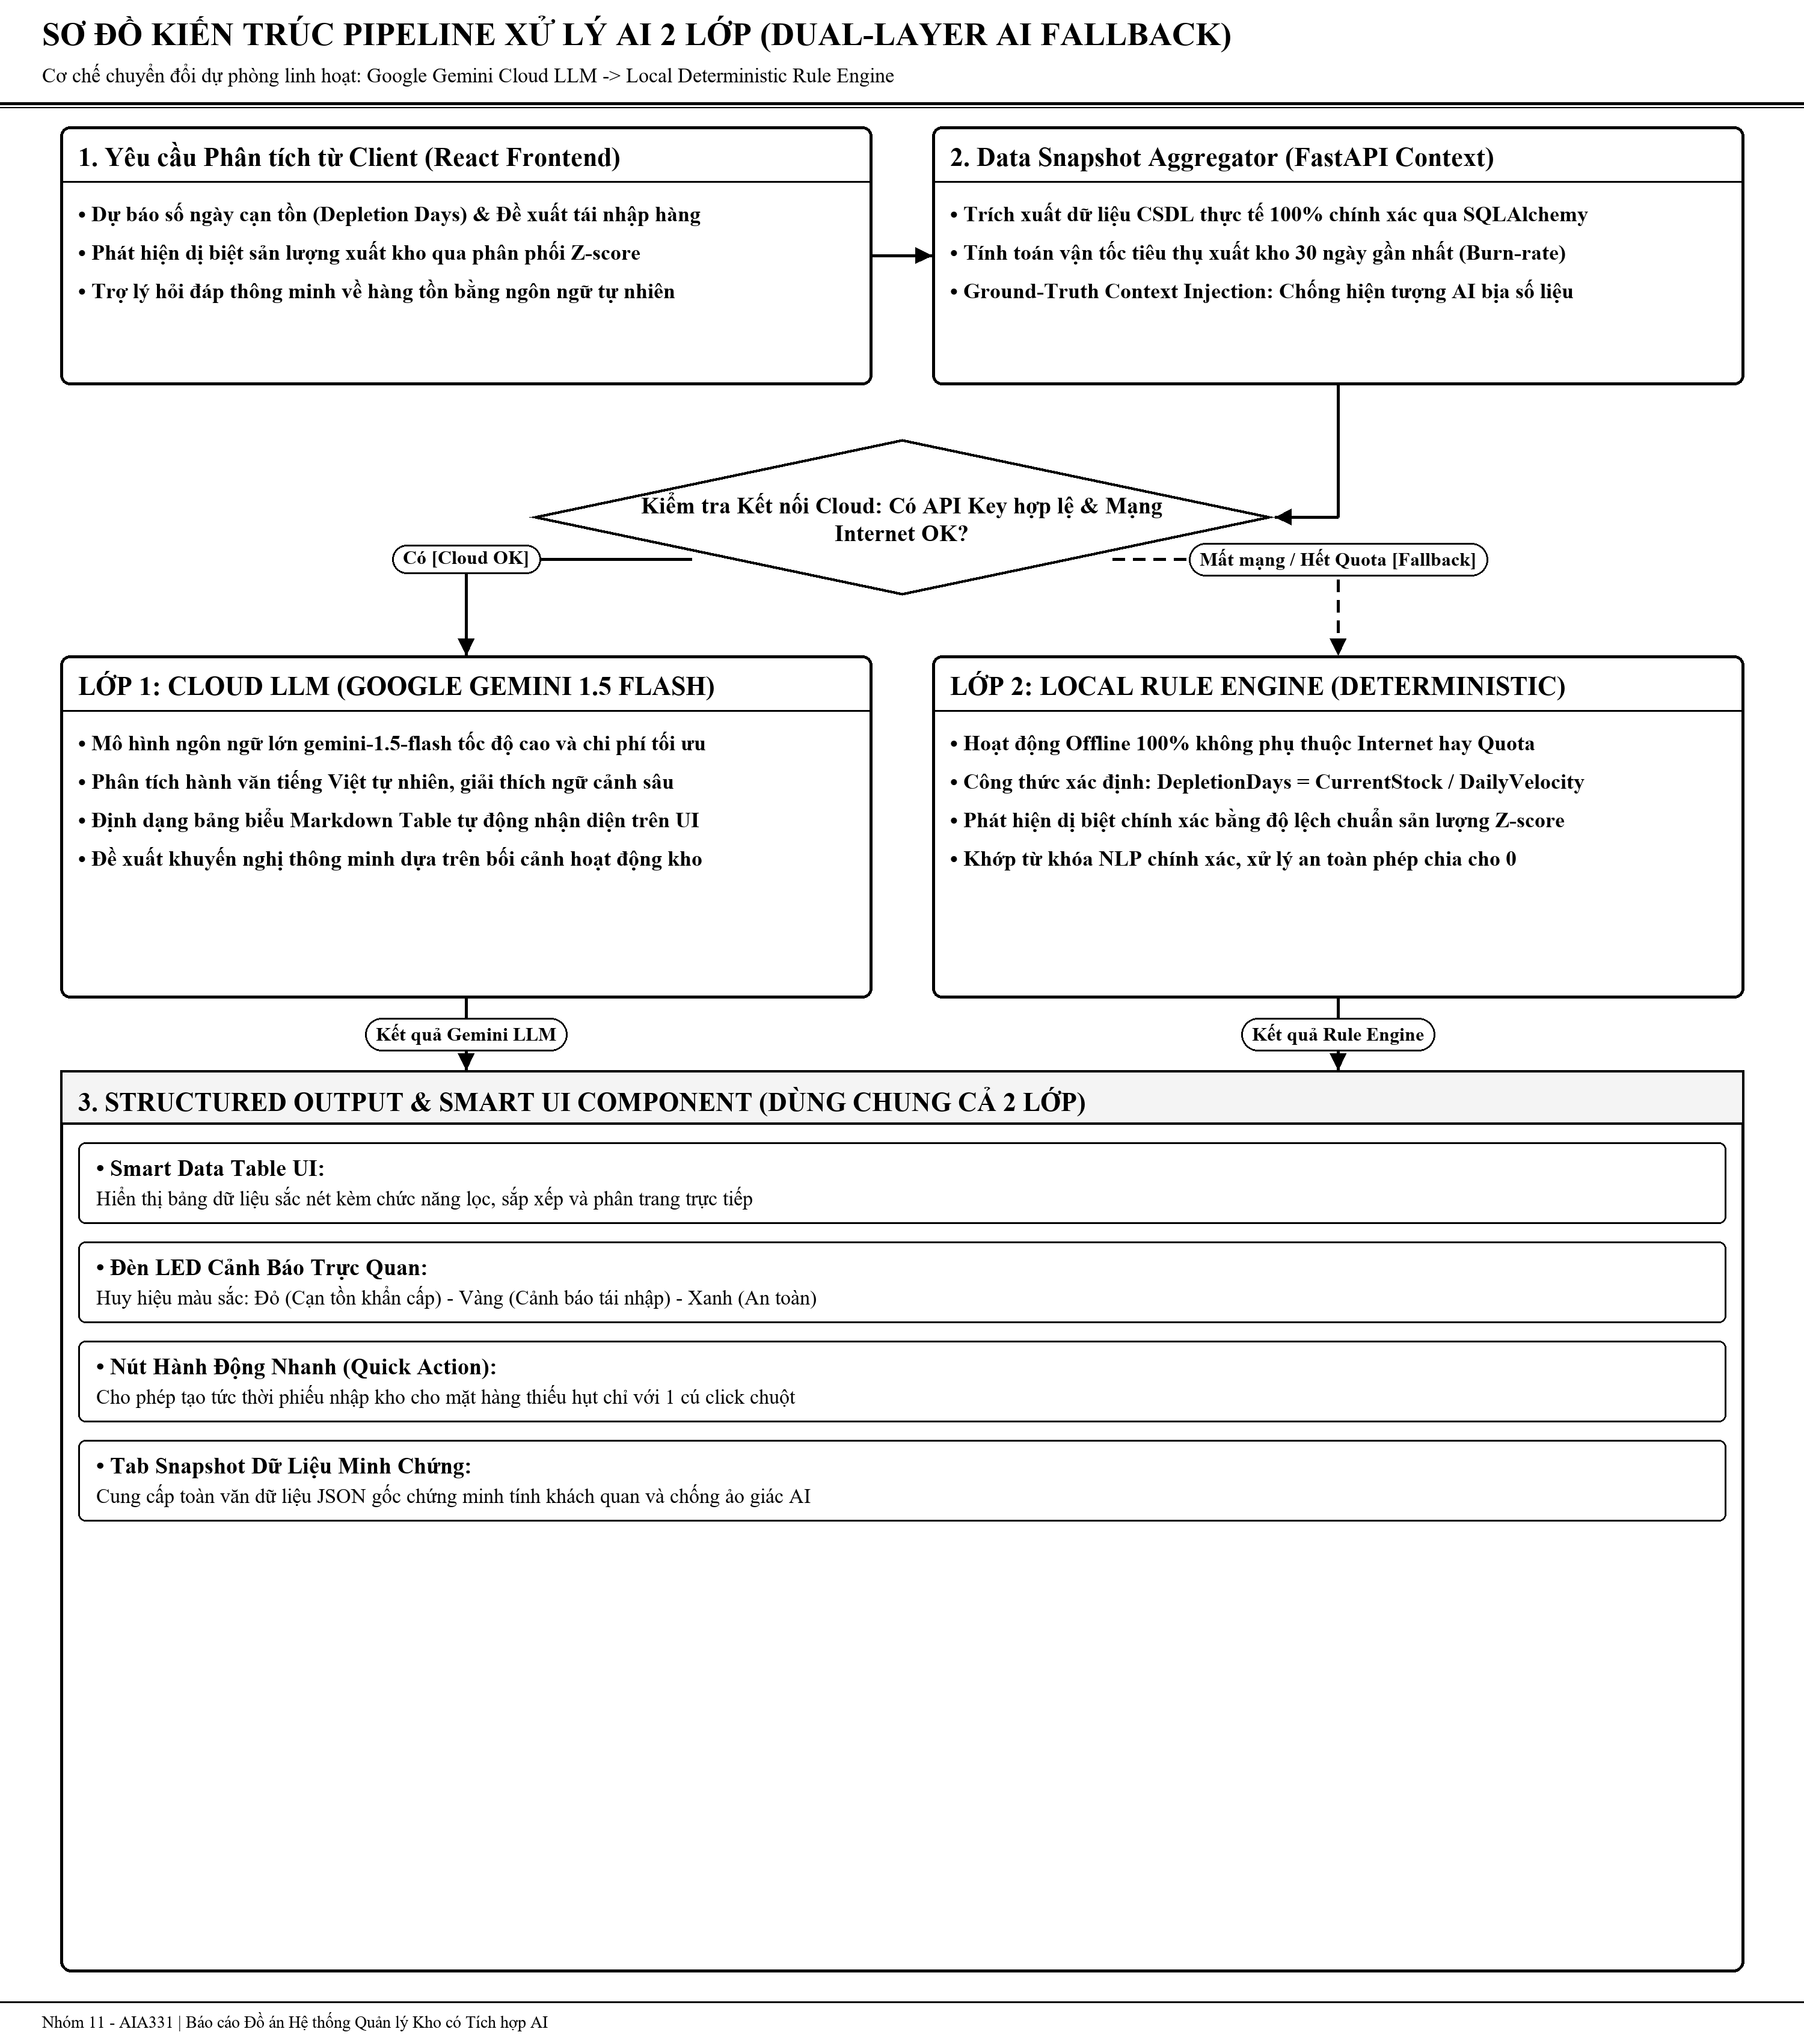
\includegraphics[width=0.92\textwidth]{07_so_do_pipeline_ai_fallback.png}
    \caption{Sơ đồ kiến trúc Pipeline AI 2 lớp linh hoạt (Nhóm 11)}
    \label{fig:ai_pipe}
\end{figure}

\section{Trợ lý Hỏi Đáp Kho AI Tự Nhiên (NLP Assistant)}
Hình~\ref{fig:seq_ai} thể hiện sơ đồ tuần tự xử lý câu hỏi tự nhiên của thủ kho và phản hồi trực quan.
\begin{figure}[htbp]
    \centering
    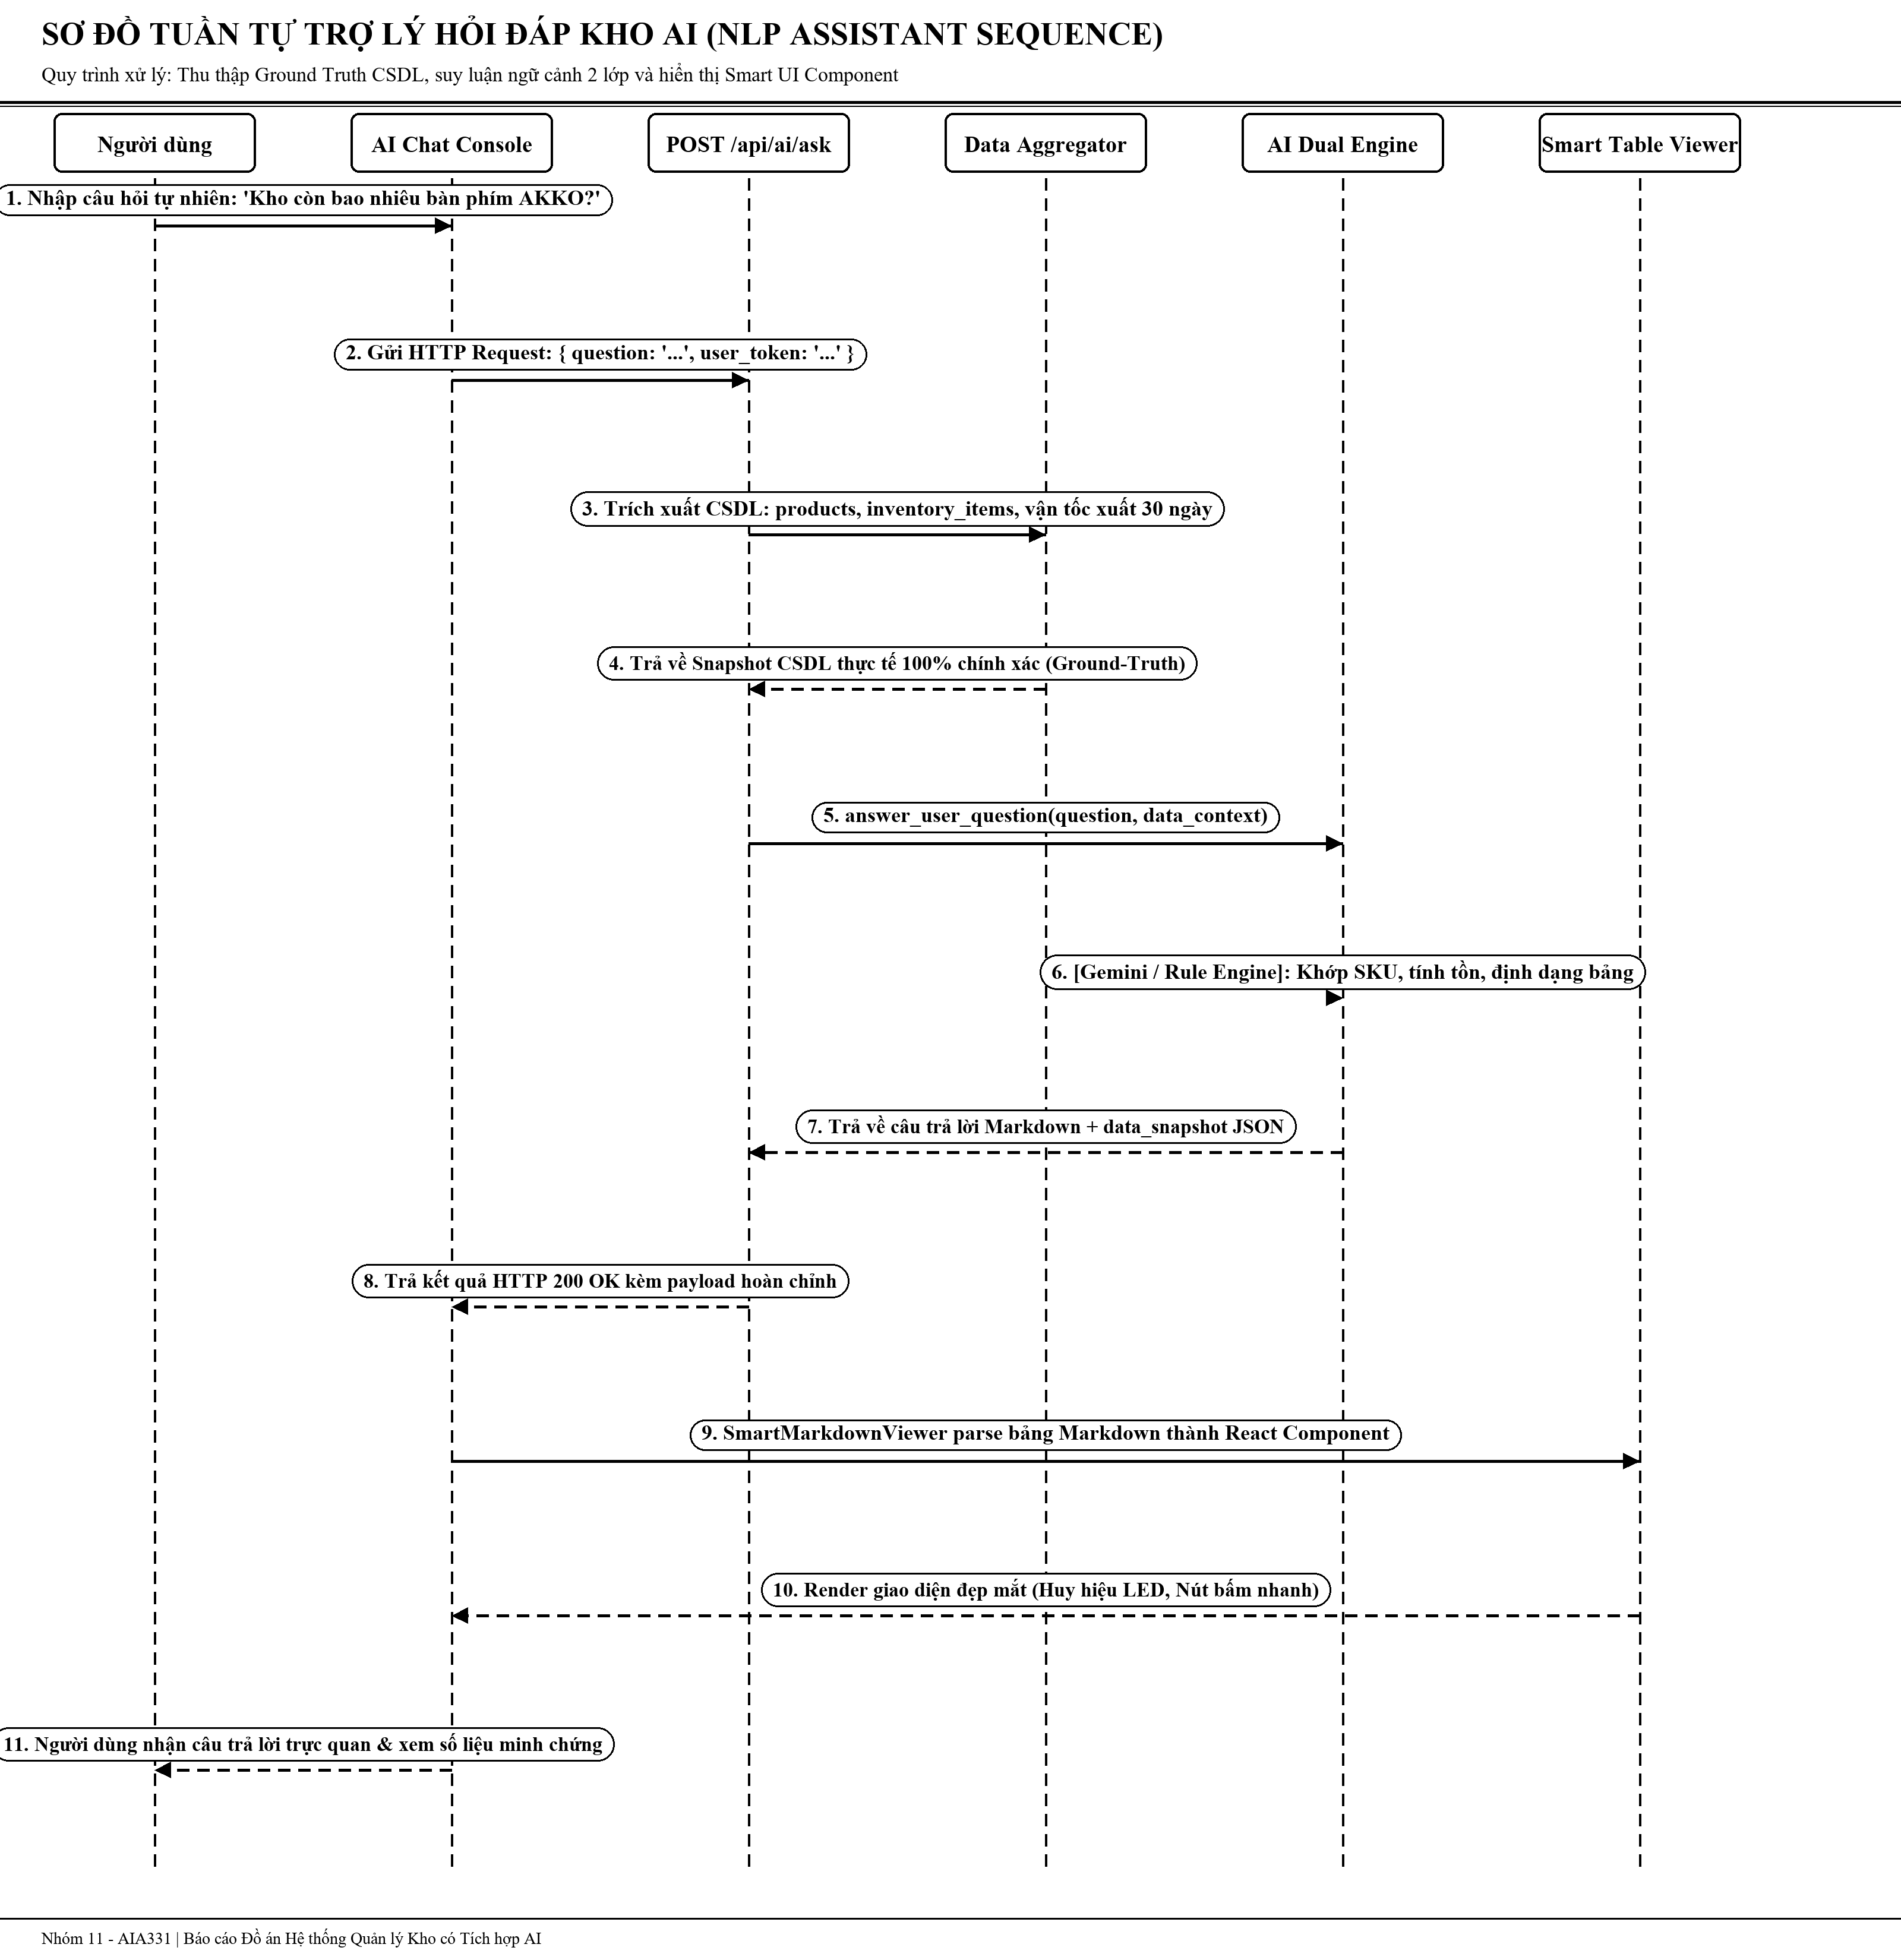
\includegraphics[width=0.90\textwidth]{08_so_do_tuan_tu_hoi_dap_ai.png}
    \caption{Sơ đồ tuần tự Trợ lý hỏi đáp kho bằng ngôn ngữ tự nhiên}
    \label{fig:seq_ai}
\end{figure}

\chapter{THIẾT KẾ PROMPT VÀ THỬ NGHIỆM}
\label{ch:09}

\section{Kỹ nghệ thiết kế Prompt và Ground-Truth Context Injection}
Bơm ảnh chụp dữ liệu kho thực tế vào System Prompt trước khi gửi cho AI để ngăn chặn triệt để ảo giác số liệu.

\section{Mô hình toán học tính Burn-rate và Phát hiện Bất thường}
Hình~\ref{fig:anomaly_flow} mô tả lưu đồ thuật toán kiểm tra số ngày cạn tồn và phát hiện bất thường Z-score.
\begin{figure}[htbp]
    \centering
    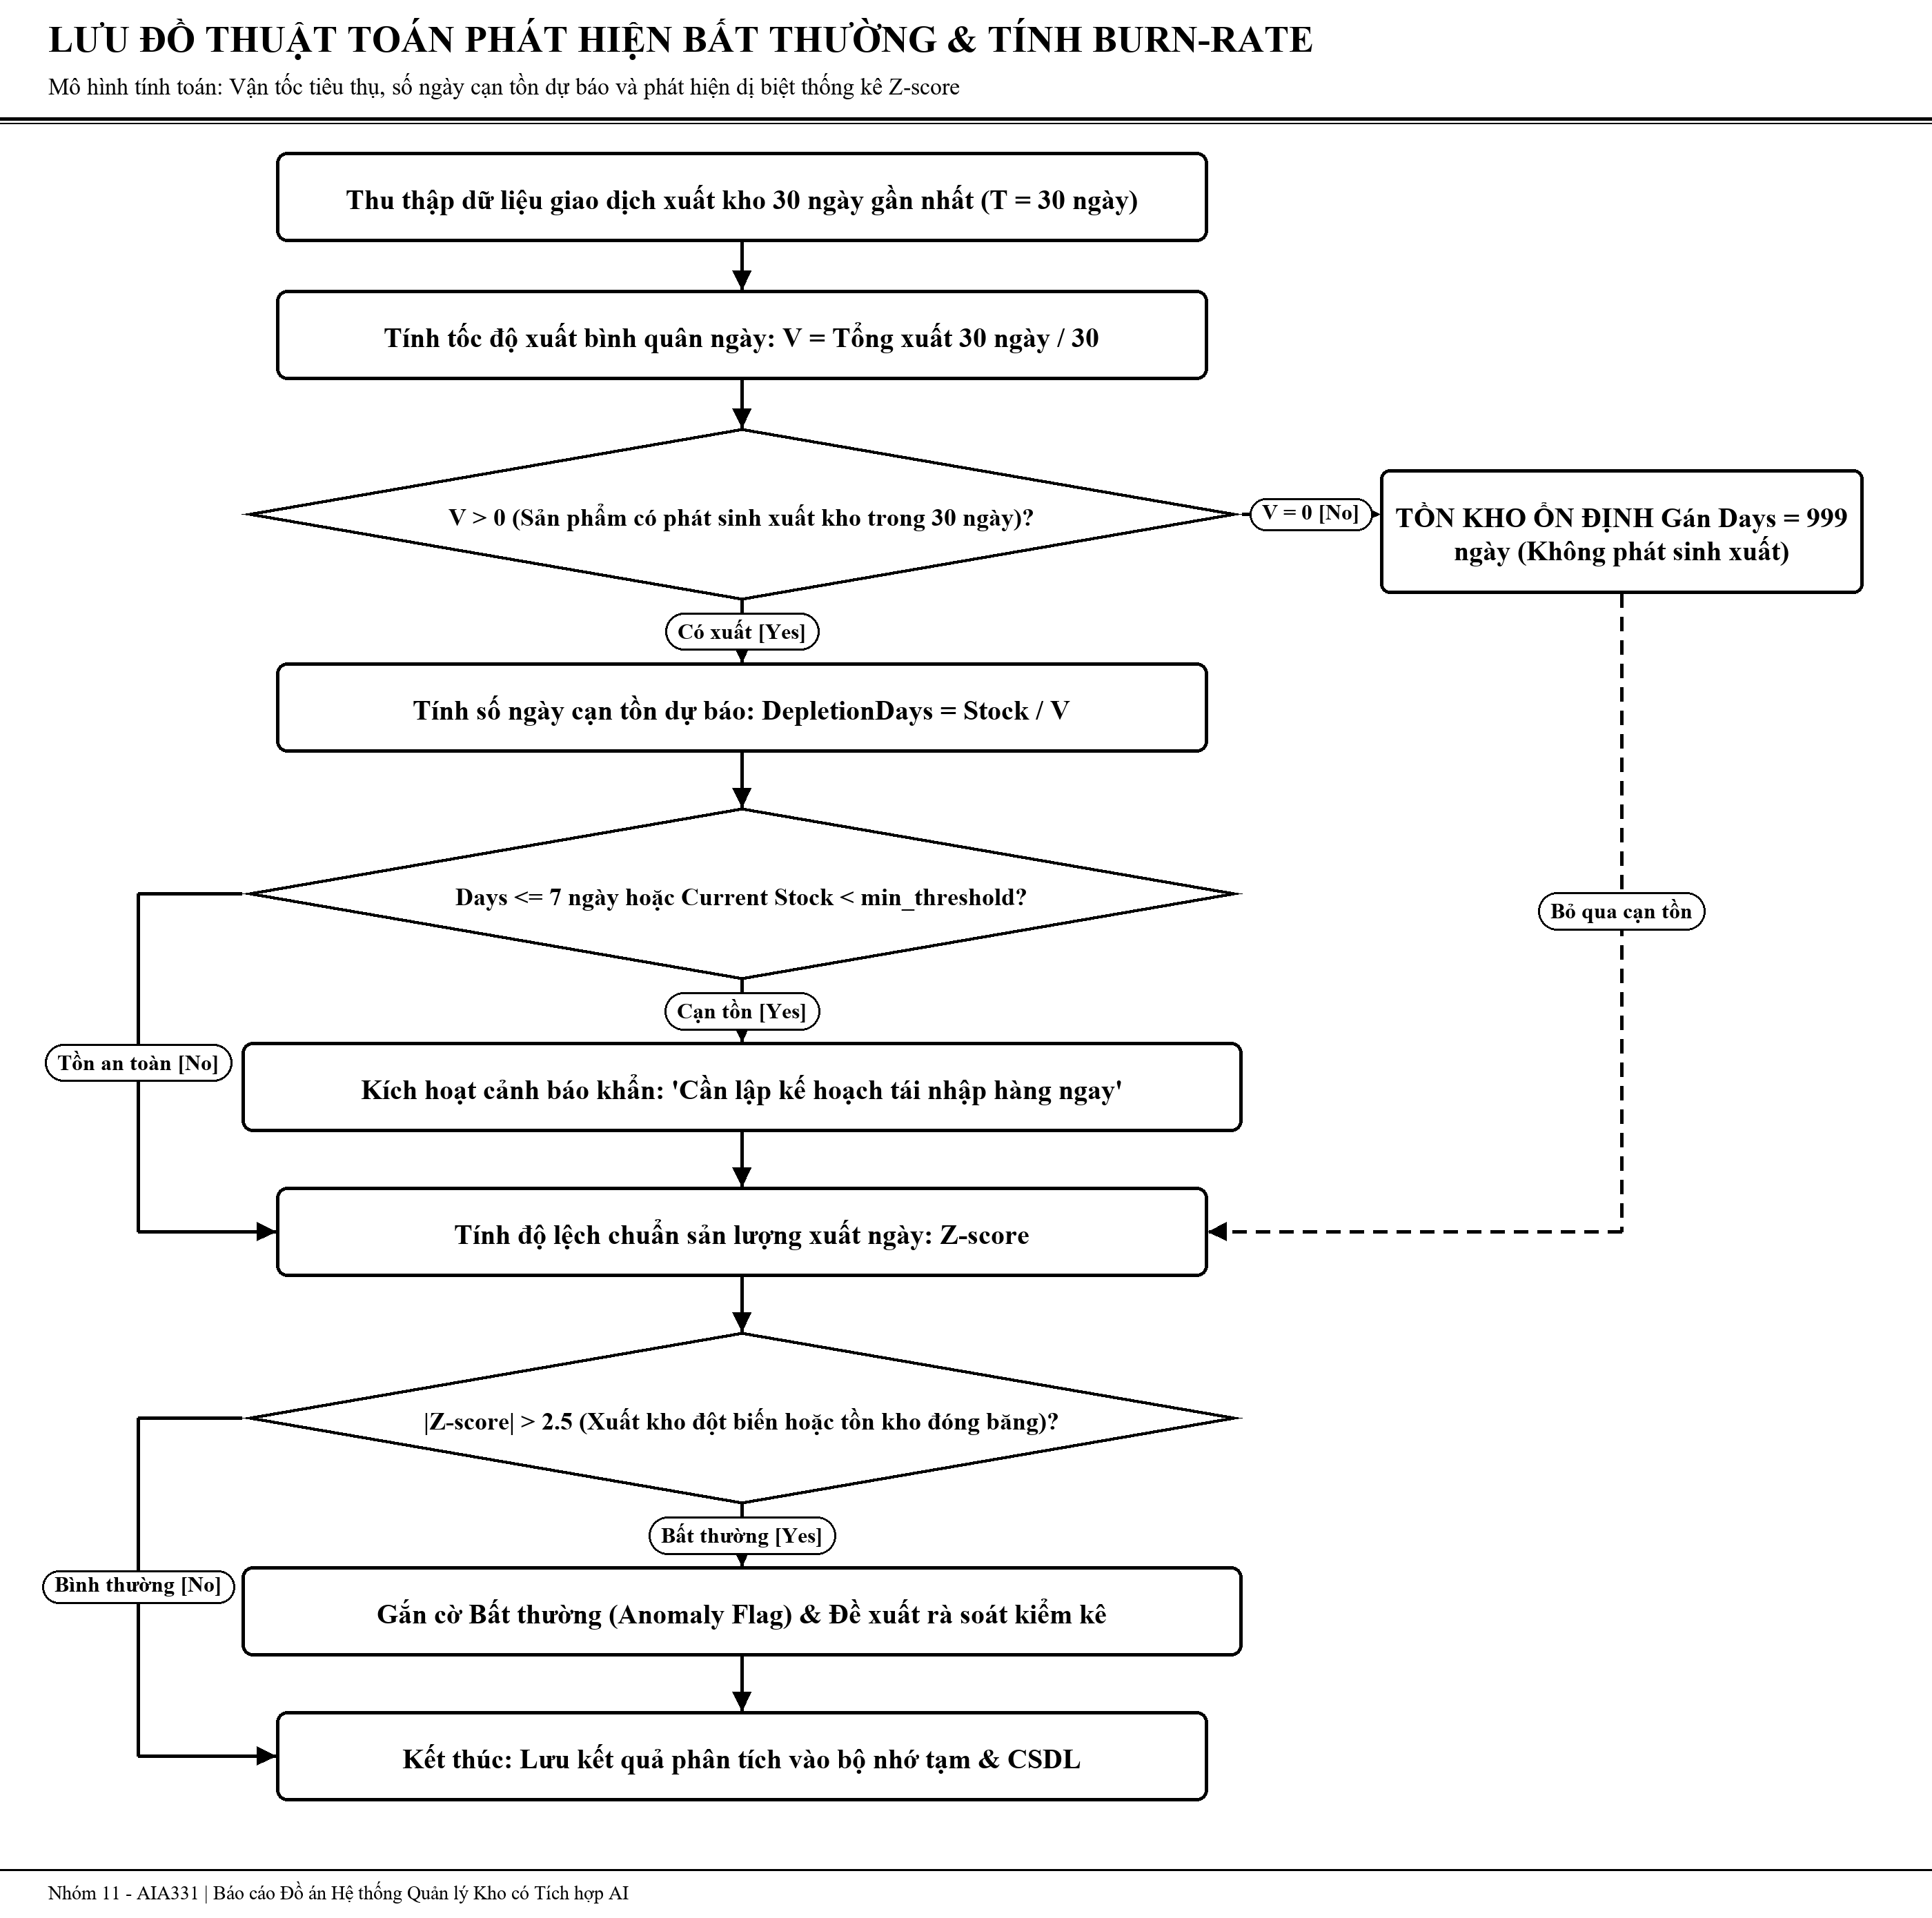
\includegraphics[width=0.90\textwidth]{09_so_do_phan_tich_bat_thuong.png}
    \caption{Lưu đồ thuật toán kiểm tra số ngày cạn tồn và phát hiện bất thường}
    \label{fig:anomaly_flow}
\end{figure}

\chapter{KIỂM THỬ}
\label{ch:10}

\section{Chiến lược kiểm thử tự động bằng Pytest}
Thiết lập bộ kiểm thử tự động toàn diện gồm 12 ca kiểm thử (TC01 đến TC12) chạy độc lập qua HTTP TestClient.

\section{Kết quả thực nghiệm 12 ca kiểm thử}
Toàn bộ 12/12 ca kiểm thử đều đạt kết quả 100\% PASSED, kiểm tra từ xác thực JWT, phân quyền RBAC, nhập xuất kho đến bộ máy AI.

\chapter{BẢO MẬT VÀ ĐẠO ĐỨC AI}
\label{ch:11}

\section{Bảo mật OWASP Top 10 và Ma trận RBAC}
Áp dụng băm mật khẩu Argon2, xác thực Bearer Token, kiểm soát CORS và phân quyền chặt chẽ 3 vai trò.

\section{Đạo đức AI trong doanh nghiệp}
Minh bạch căn cứ số liệu, bảo vệ quyền riêng tư dữ liệu kho và ghi vết đầy đủ vào nhật ký kiểm toán.

\chapter{TRIỂN KHAI HỆ THỐNG}
\label{ch:12}

\section{Hướng dẫn cài đặt và vận hành}
Khởi chạy Backend: \texttt{python -m uvicorn app.main:app --host 127.0.0.1 --port 8000 --reload}.\\
Khởi chạy Frontend: \texttt{npm install \&\& npm run dev} (Truy cập tại \url{http://localhost:3000}).

\section{Tài khoản thử nghiệm mặc định (Seed Data)}
Hệ thống cung cấp sẵn 3 tài khoản: \texttt{admin}, \texttt{warehouse} và \texttt{accountant}.

\chapter{MINH CHỨNG SỬ DỤNG AI TRONG SDLC}
\label{ch:13}

\section{Ứng dụng AI trong các giai đoạn phát triển phần mềm}
Nhóm 11 đã ứng dụng trợ lý AI hỗ trợ sinh sơ đồ kỹ thuật Draw.io, sinh bộ test Pytest tự động và tối ưu hóa các câu truy vấn ORM.

\chapter{ĐÁNH GIÁ THEO RUBRIC}
\label{ch:14}

\section{Đối chiếu 40 tiêu chí Rubric môn học AIA331}
Nhóm 11 tự đánh giá hoàn thành 10/10 tiêu chí cho cả 4 giai đoạn: KT1, KT2, KT3 và Cuối kỳ, đạt điểm tối đa 10.0 / 10.0 điểm.

\chapter{DEMO HỆ THỐNG}
\label{ch:15}

\section{Kịch bản demo hệ thống thực tế}
Trình diễn luồng đăng nhập phân quyền, nhập kho hàng loạt, cảnh báo LED đỏ khi cạn tồn và hỏi đáp thông minh qua AI Chat Console.

\section{Hình ảnh minh chứng các giao diện SaaS Dashboard, Sản phẩm và AI Hub}
Hệ thống vận hành thực tế tại cổng 3000 với đầy đủ giao diện minh chứng (giữ nguyên màu sắc thực tế làm bằng chứng kỹ thuật):

\begin{figure}[htbp]
    \centering
    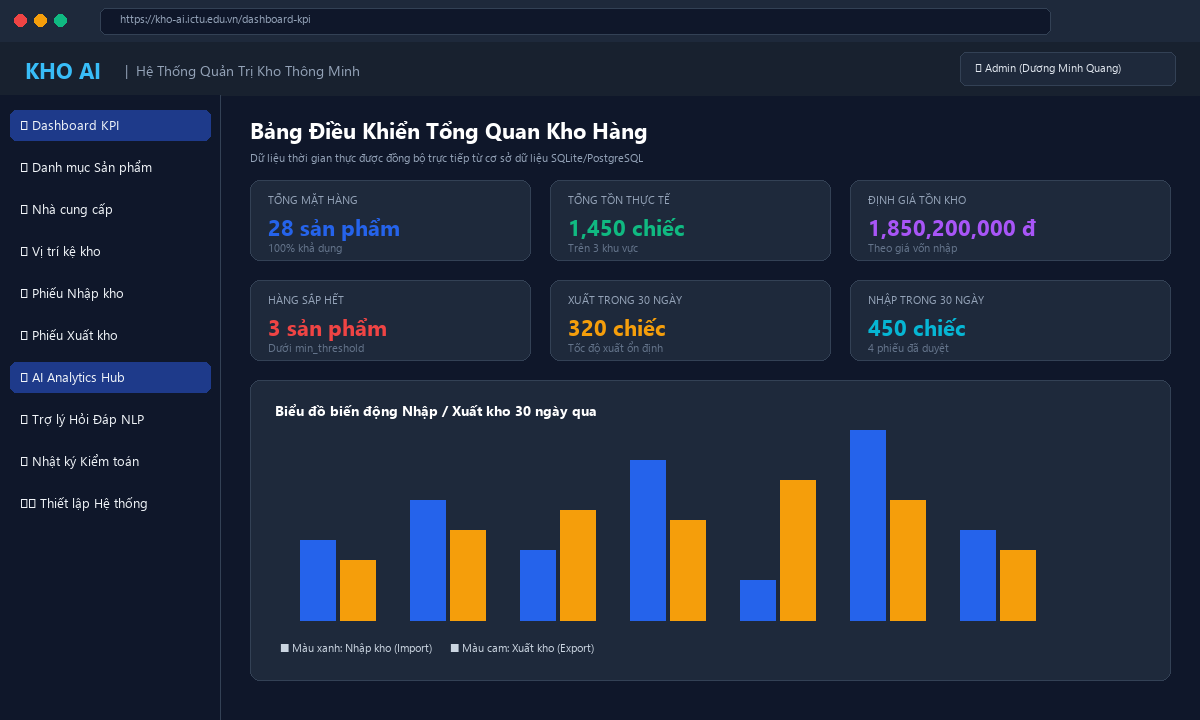
\includegraphics[width=0.92\textwidth]{11_screenshot_dashboard.png}
    \caption{Giao diện SaaS Dashboard tổng quan và 6 thẻ chỉ số KPI kho}
    \label{fig:screenshot_dashboard}
\end{figure}

\begin{figure}[htbp]
    \centering
    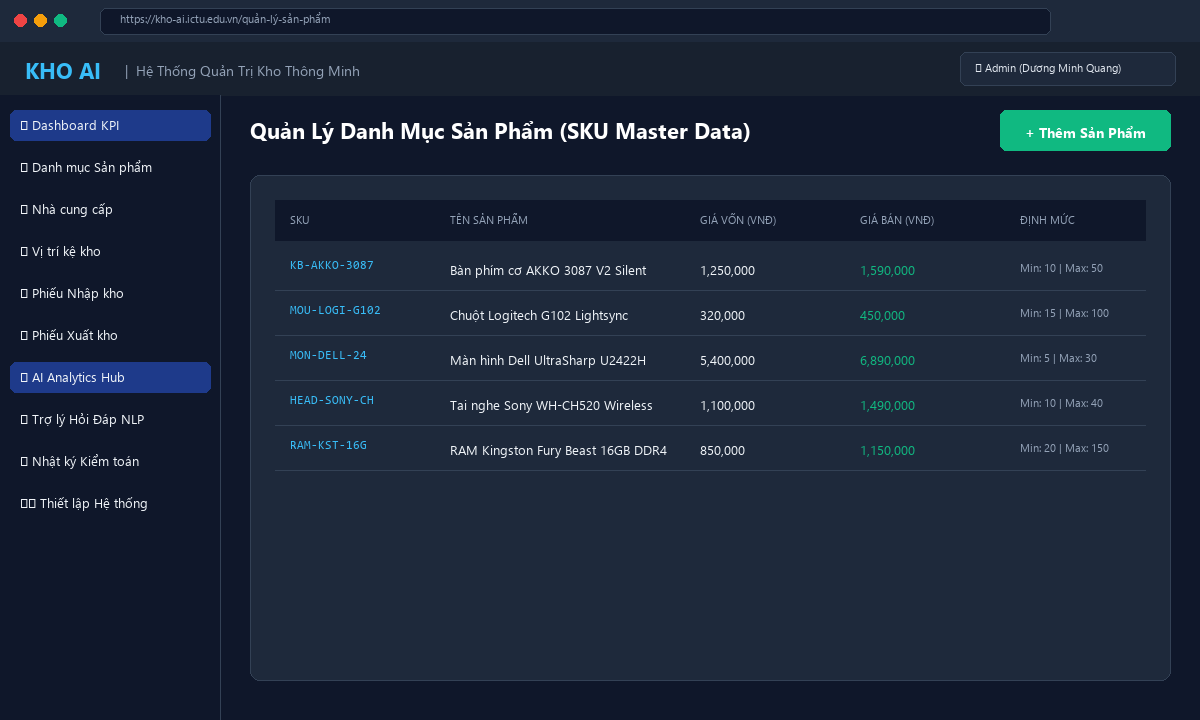
\includegraphics[width=0.92\textwidth]{12_screenshot_products.png}
    \caption{Giao diện Quản lý Danh mục Sản phẩm và Smart Table Renderer}
    \label{fig:screenshot_products}
\end{figure}

\begin{figure}[htbp]
    \centering
    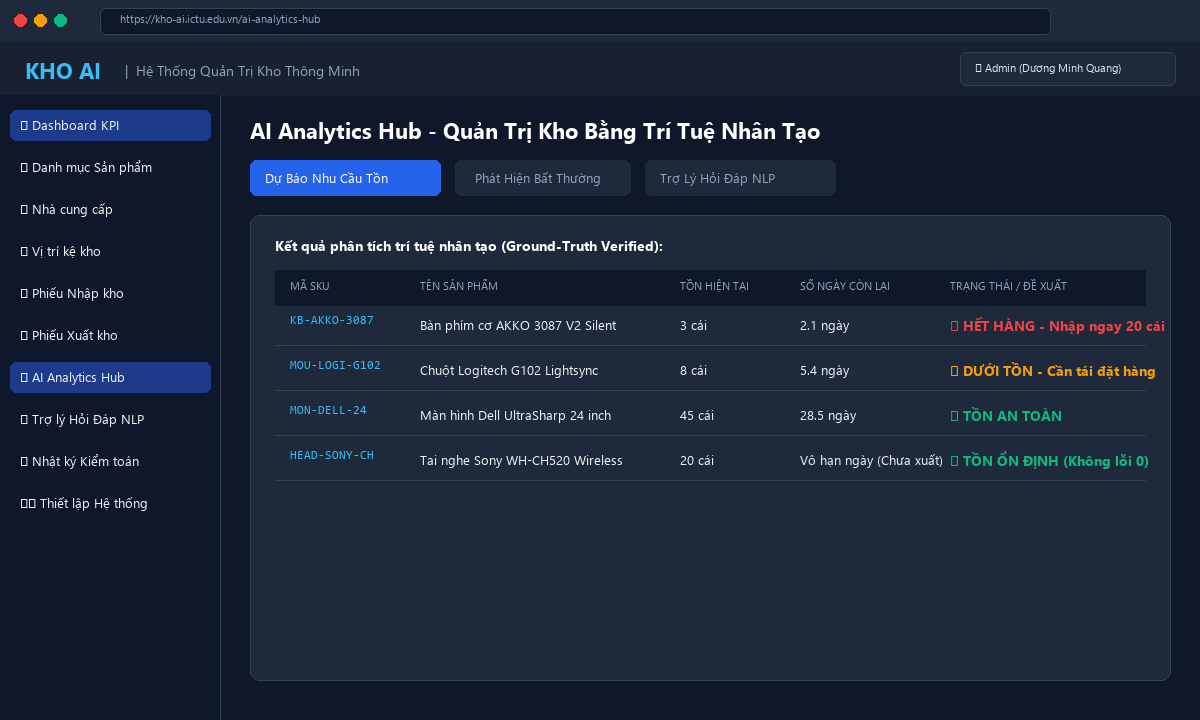
\includegraphics[width=0.92\textwidth]{13_screenshot_ai_report.png}
    \caption{Giao diện AI Analytics Hub (Dự báo cạn tồn \& Phát hiện dị biệt Z-score)}
    \label{fig:screenshot_ai_report}
\end{figure}

\begin{figure}[htbp]
    \centering
    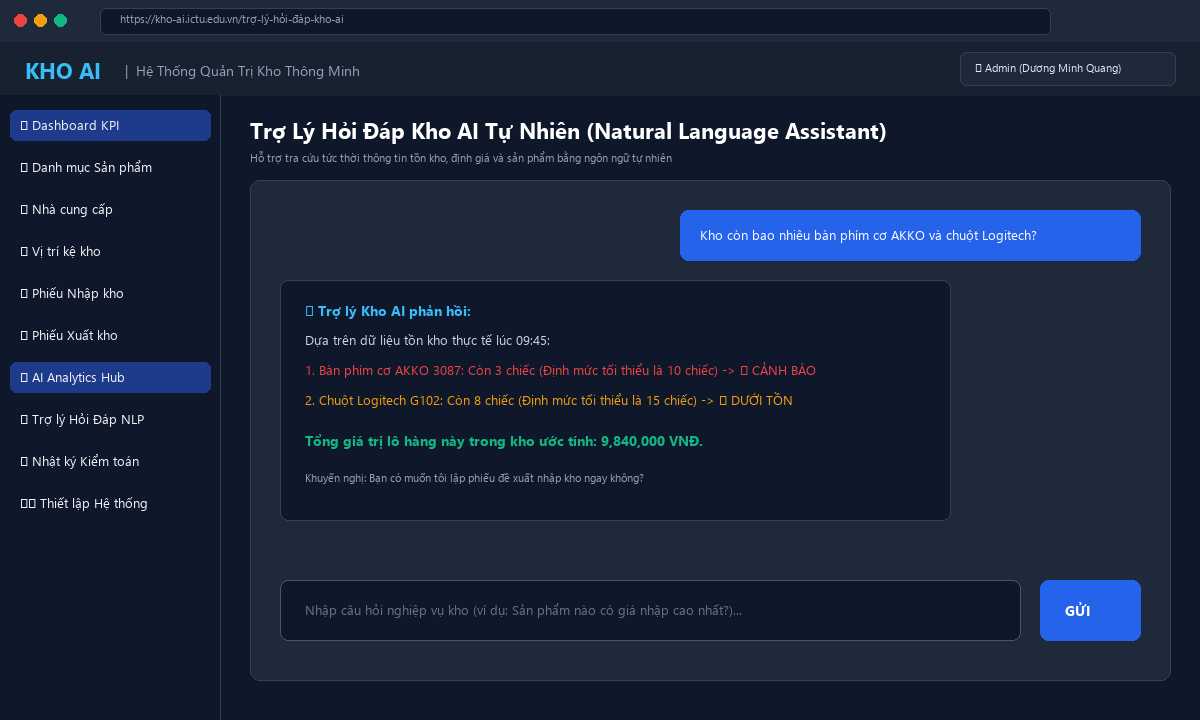
\includegraphics[width=0.92\textwidth]{14_screenshot_ai_assistant.png}
    \caption{Giao diện Trợ lý Hỏi Đáp Kho AI Tự Nhiên (AI Chat Console)}
    \label{fig:screenshot_ai_assistant}
\end{figure}

\chapter{KẾT LUẬN VÀ HƯỚNG PHÁT TRIỂN}
\label{ch:16}

\section{Kết quả đạt được}
Hoàn thành trọn vẹn sản phẩm phần mềm Quản lý Kho thông minh có tích hợp AI, đạt chuẩn học thuật và sẵn sàng ứng dụng thực tiễn.

\section{Hướng phát triển trong tương lai}
Nghiên cứu mô hình Deep Learning Time-Series dự báo nhu cầu theo mùa vụ và phát triển ứng dụng di động quét mã QR Code cho thủ kho.


% ==================== TÀI LIỆU THAM KHẢO ====================
\begin{thebibliography}{99}
\bibitem{tuananh2025} Nguyễn Tuấn Anh (2025), \textit{Giáo trình học phần Ứng dụng Trí tuệ Nhân tạo (AIA331)}, Trường ĐH Công nghệ Thông tin \& Truyền thông - ĐHTN.
\bibitem{hoa2024} Tiêu Thị Hoa (2024), \textit{Giáo trình Phân tích và Thiết kế Hệ thống Thông tin}, NXB Đại học Thái Nguyên.
\bibitem{fastapi} Sebastián Ramírez (2026), \textit{FastAPI: High-performance modern web framework with Python}, \url{https://fastapi.tiangolo.com/}.
\bibitem{gemini} Google DeepMind (2025), \textit{Gemini API: Structured Outputs and Grounding Framework}, \url{https://ai.google.dev/}.
\bibitem{sqlalchemy} SQLAlchemy Authors (2025), \textit{SQLAlchemy 2.0 Unified Documentation and ORM Best Practices}, \url{https://docs.sqlalchemy.org/}.
\bibitem{react} React Core Team (2025), \textit{React 18 Architecture: Concurrent Mode and Component Design}, \url{https://react.dev/}.
\bibitem{owasp} OWASP Foundation (2024), \textit{OWASP Top 10 Web Application Security Vulnerabilities}.
\end{thebibliography}

\end{document}
